\section{Signal extraction}
%%%%%%%%%%%%%%%%%%%%%%%%%%%%%%%%%%%%%%%%%%%%%%%%%%%%%%%%%%%%%%%%%%%%%%
\label{sec:SignalExtraction}

In this section the fitting procedure as well as the measured signal and background yields are described.


\subsection{Fitting procedure}\label{sec:fit}

The signal, including ggH, VBF, and VH production mechanisms, is extracted in each bin of \pth{} by performing a binned maximum likelihood fit simultaneously in all \pth bins to a two-dimensional template for signal and background in the \mll--\mt plane.
The variables used for the two-dimensional template are chosen for their power to discriminate signal and background contributions. This is shown in Fig.~\ref{fig:2Dlegacy}, where the two-dimensional simulated distributions are shown for the signal and background processes in the 0 jets category. As can be observed, the signal contribution in the 0 jets category is mostly distributed in the low \mll region and for \mt values around 90--110\GeV. The background contribution, which is mainly owed to the WW, W+jets and \dytt production, is instead distributed in the high \mll region and for intermediate values of \mt (below 100\GeV).

\begin{figure}[htb]
\centering
\subfigure[]{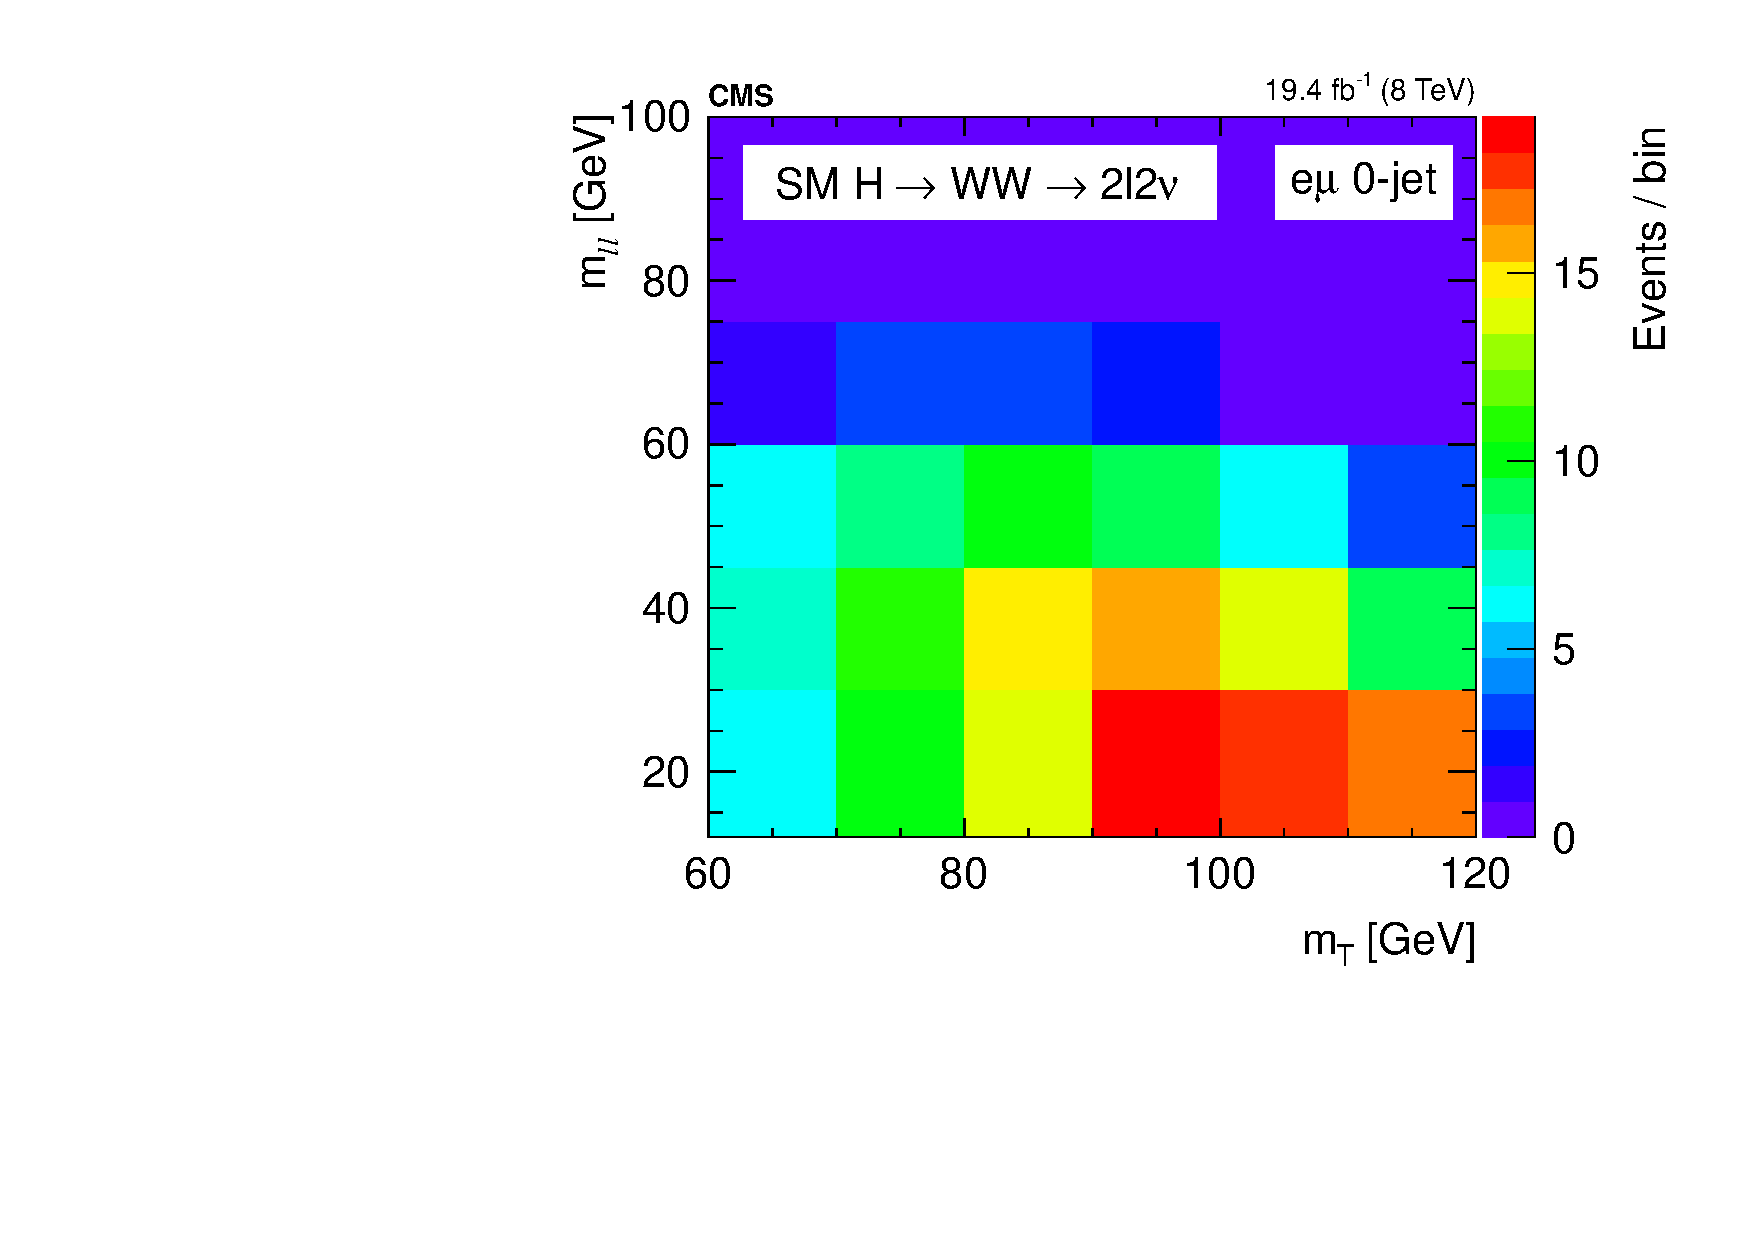
\includegraphics[width=0.45\textwidth]{images/legacyPlots/2d_prefit_0j_125_sig_paper.pdf}}
\subfigure[]{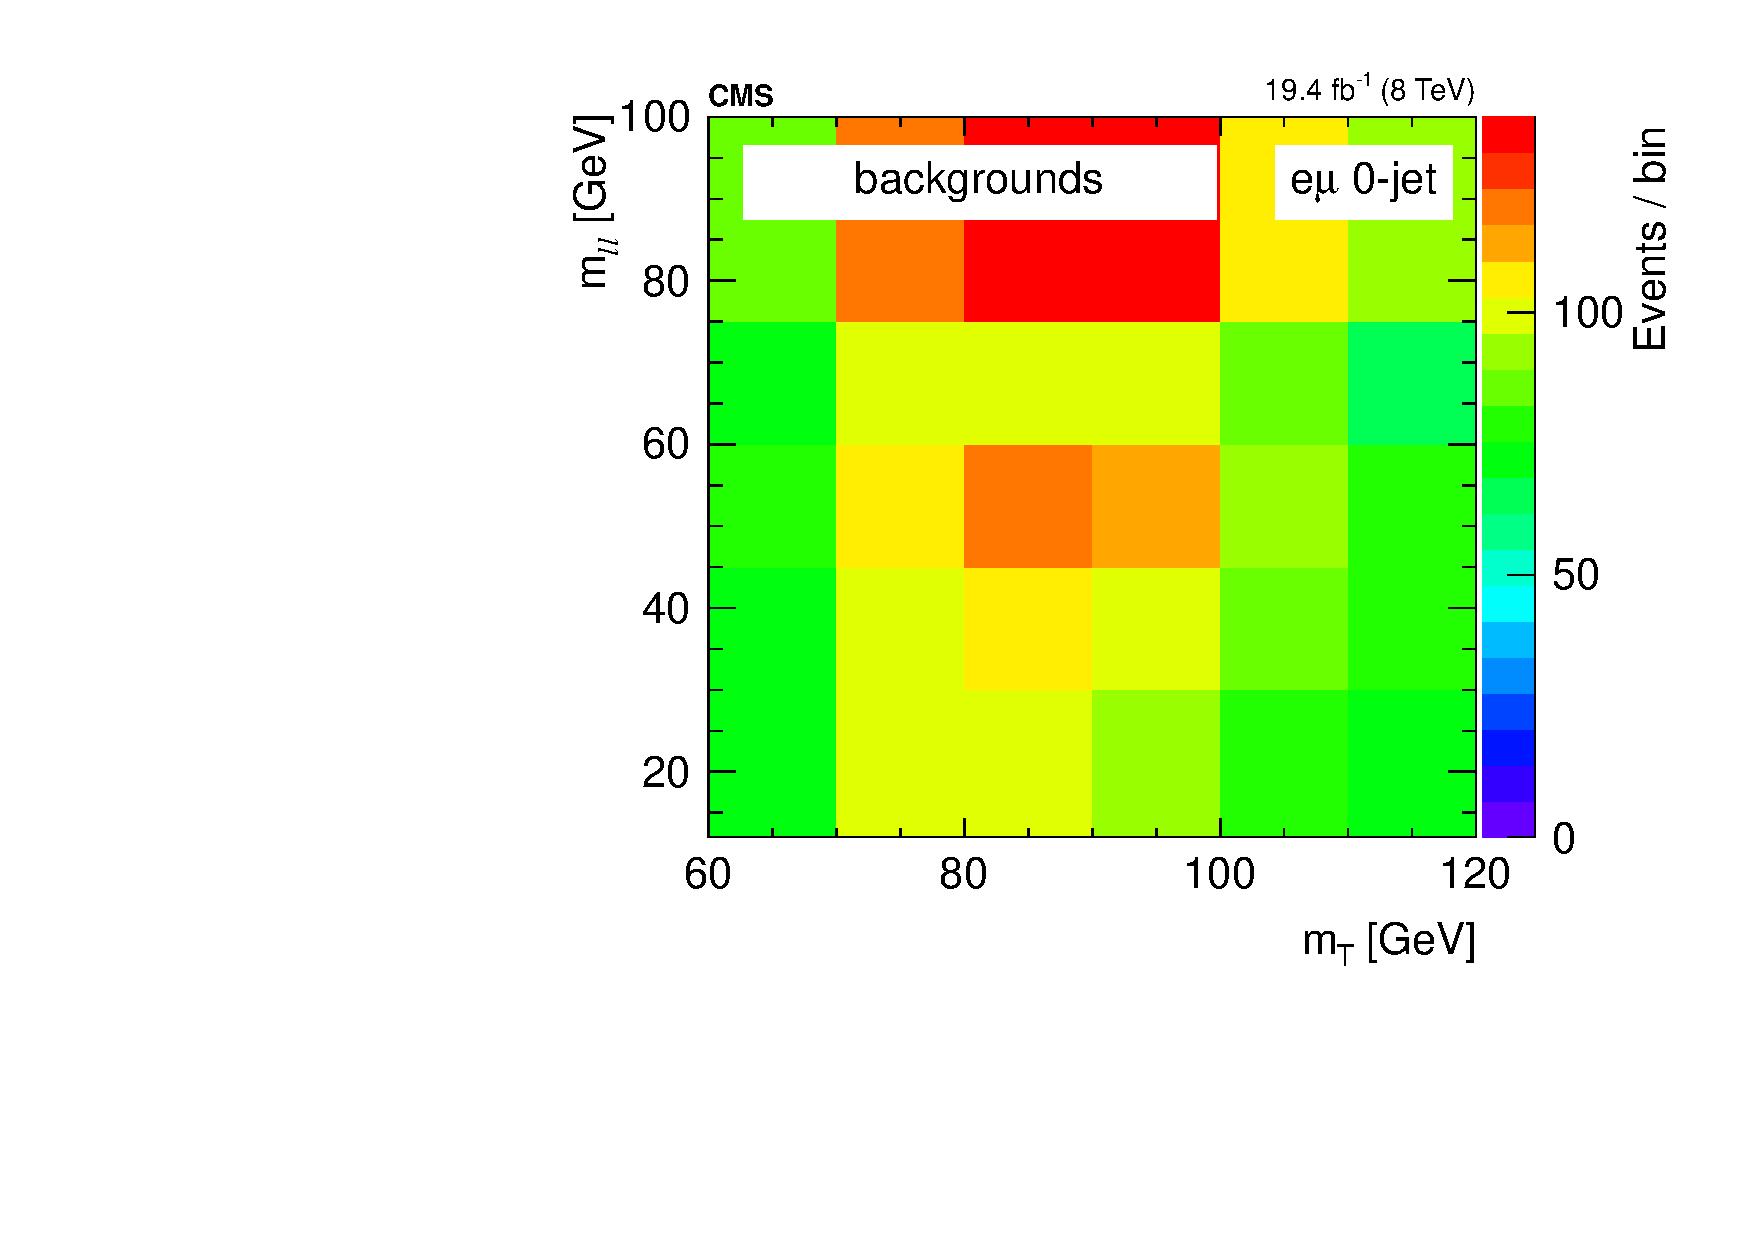
\includegraphics[width=0.45\textwidth]{images/legacyPlots/2d_prefit_0j_125_bkg_paper.pdf}}
\caption{Two-dimensional \mll--\mt distribution for signal (a) and background (b) processes in the 0 jets category.\label{fig:2Dlegacy}}
\end{figure}

Six different signal strengths are extracted from the fit, one for each \pth~bin. The relative contributions of the different Higgs production mechanisms in the signal template are taken to be the same as in the SM. The sources of systematic uncertainty are considered as nuisance parameters in the fit.

The binning of the \mll and \mt templates is chosen to be:
\begin{itemize}
\item {\mll: $[12,30,45,60,75,100,125,150,175,200]$} 
\item {\mt: $[60,70,80,90,100,110,120,140,160,180,200,220,240,280]$}
\end{itemize}

To avoid a dependence of the results on the variables used for the template fit, \mll and \mt need to be uncorrelated with respect to \pth.
This has been verified and the correlation between the discriminating variables and \pth is shown in Fig.~\ref{fig:correlation_ggH} and Fig.~\ref{fig:correlation_vbf} for ggH and VBF production modes, respectively.

\begin{figure}[htb]
\centering
\subfigure[]{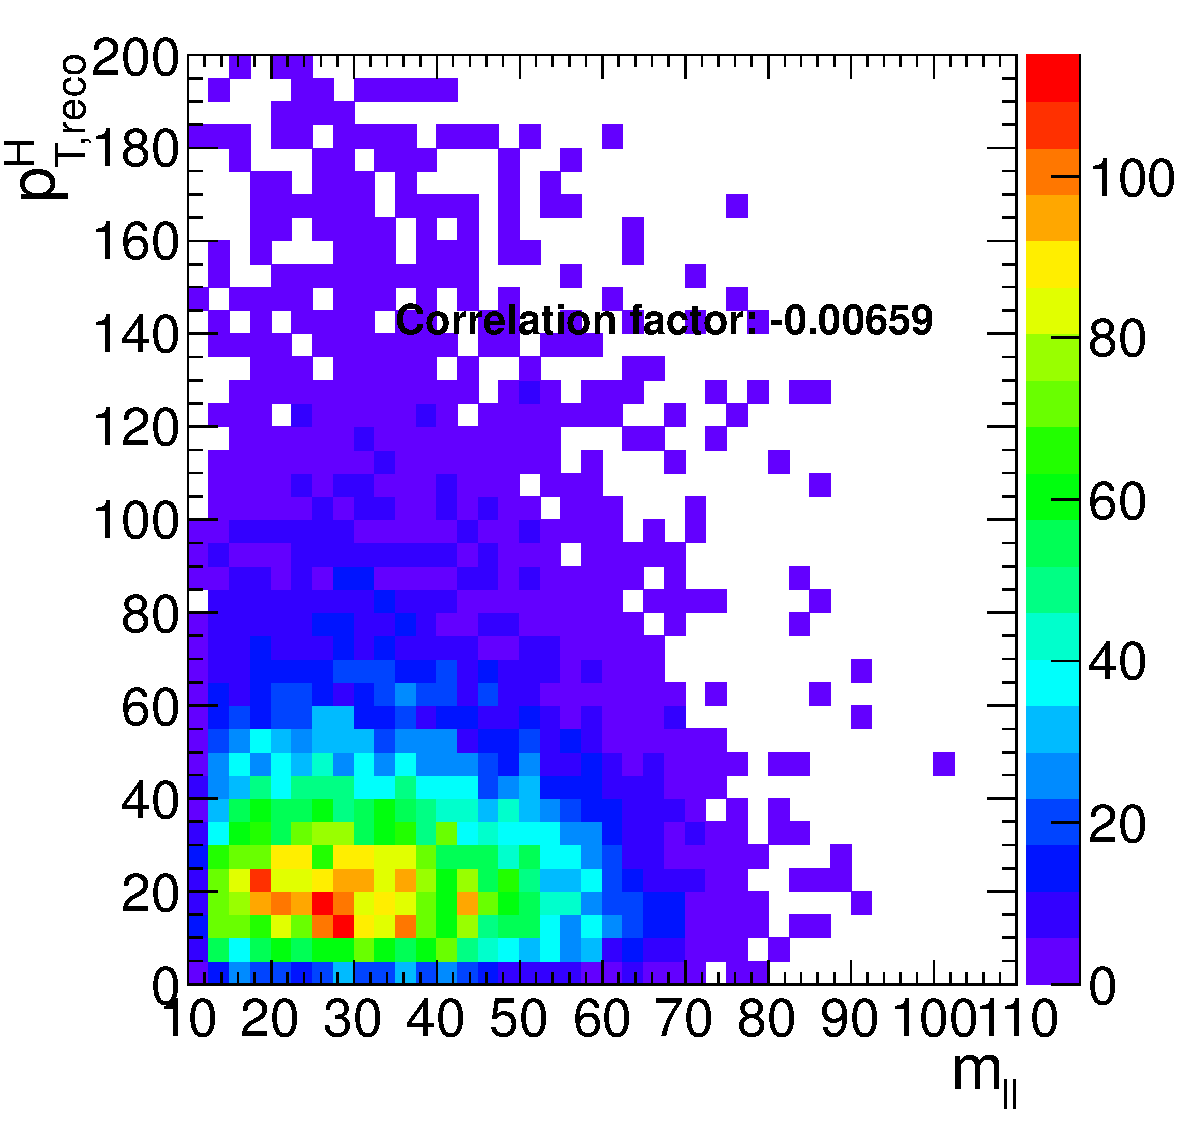
\includegraphics[width=0.45\textwidth]{images/correlationmll_ggH.pdf}}
\subfigure[]{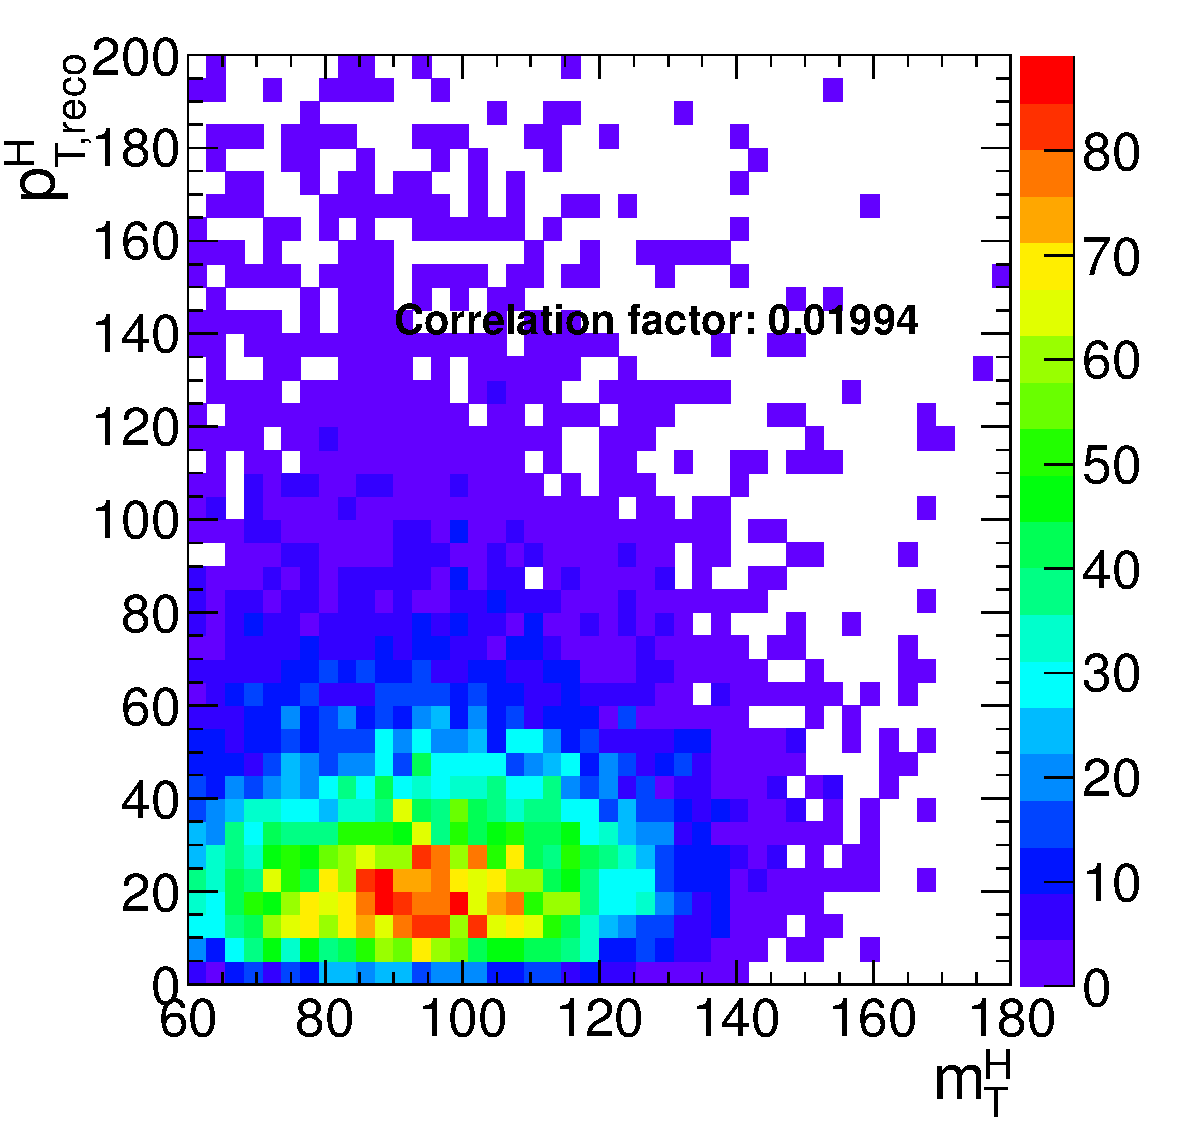
\includegraphics[width=0.45\textwidth]{images/correlationmth_ggH.pdf}}
\caption{Correlation between $\pth$ and $\mll$ (a) and between \pth and \mt (b) after the full selection for the ggH production mode.\label{fig:correlation_ggH}}
\end{figure}

\begin{figure}[htb]
\centering
\subfigure[]{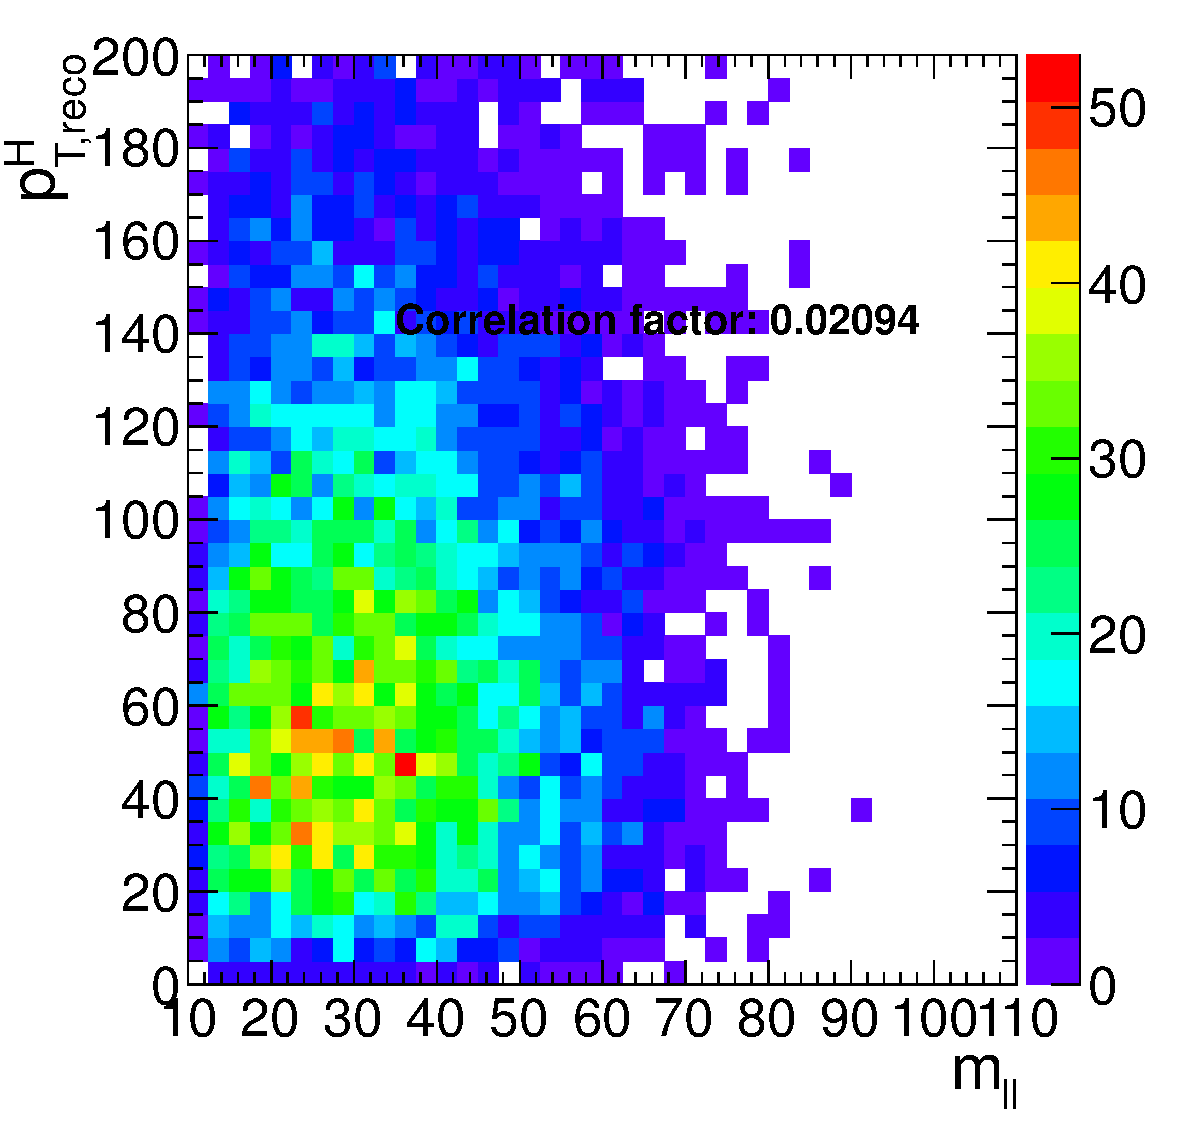
\includegraphics[width=0.45\textwidth]{images/correlationmll_vbf.pdf}}
\subfigure[]{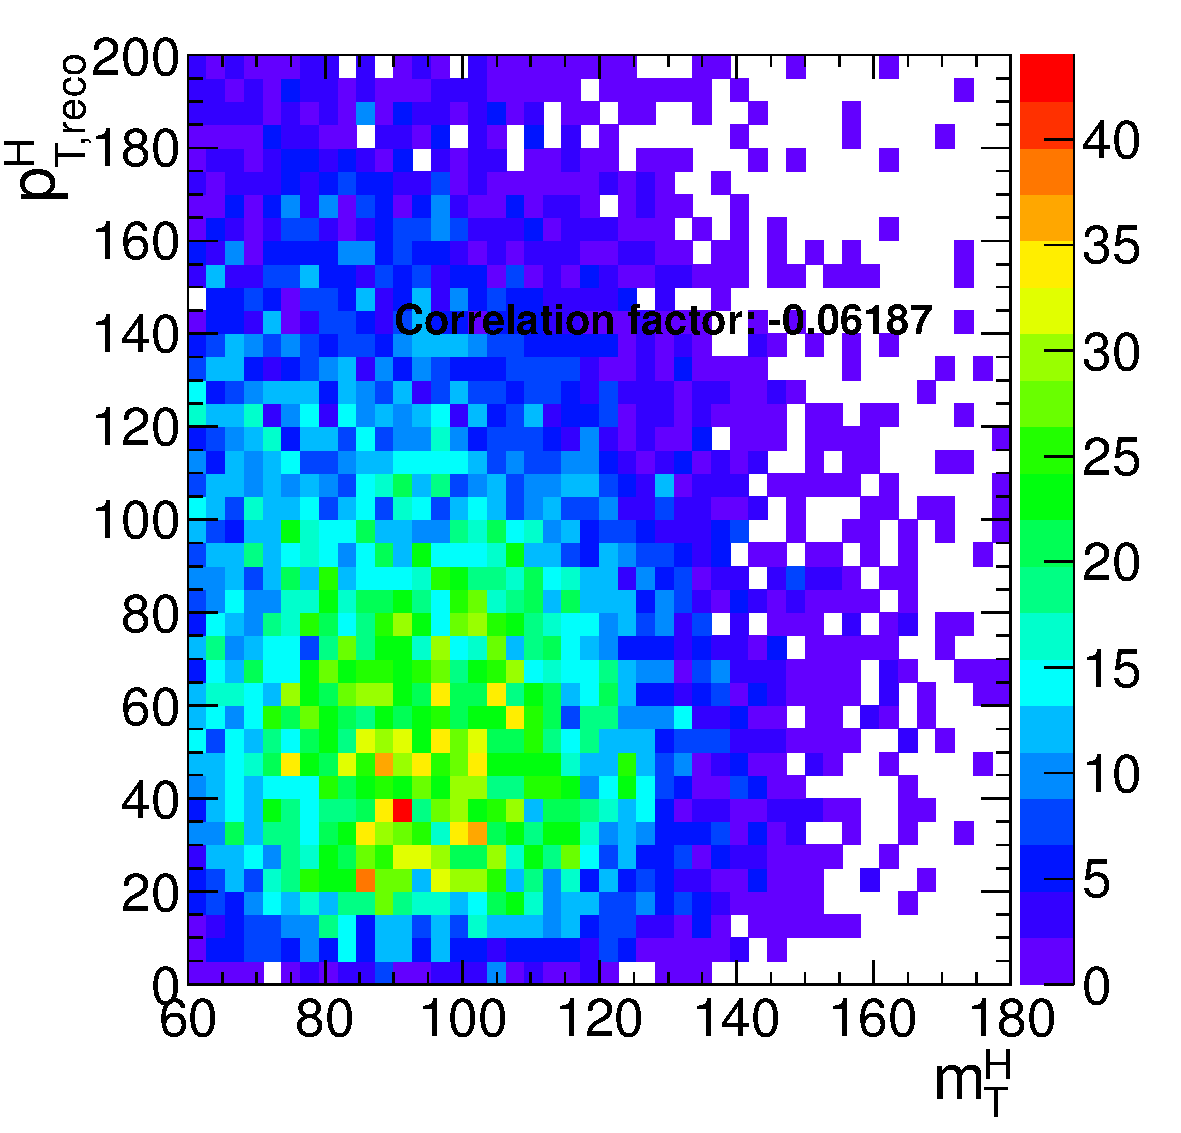
\includegraphics[width=0.45\textwidth]{images/correlationmth_vbf.pdf}}
\caption{Correlation between \pth and \mll (a) and between \pth and \mt (b) after the full selection for the VBF production mode.\label{fig:correlation_vbf}}
\end{figure}

The signal strength $\mu$ in each bin, defined as the ratio between the measured cross section and the SM one, $\mu = \sigma/\sigma_\mathrm{SM}$, is allowed to float between -10 and +10, thus allowing negative values. This is mainly intended to allow future combinations with similar measurements without introducing any bias.

Because of detector resolution effects, some of the reconstructed $\hww$ signal events might originate from outside the fiducial phase space.  
These out-of-fiducial signal events cannot be precisely handled by the unfolding procedure and must be subtracted from the reconstructed spectrum. The \pth distribution of the out-of-fiducial signal events is taken from simulation, and each bin is multiplied by the corresponding measured signal strength before performing the subtraction. 

At the end, the number of events in each bin $i$ of the measured spectrum is:
\begin{equation}\label{eq:sig_yield}
N_i = \mu_i (s_i -f_i) \quad ,
\end{equation}

\noindent where $\mu_i$ is the measured signal strength, $s_i$ and $f_i$ are respectively the total number of reconstructed signal events and the number of reconstructed out-of-fiducial signal events expected from simulation.

The fit makes use of the binned maximum likelihood approach. The likelihood function, $\mathcal{L}$, restricted to the \pth bin $j$, can be written as:
\begin{equation}
\mathcal{L}(\mu_j,\theta) = \prod_{i=0}^{N_\mathrm{bins}} \frac{(\mu_j s_i(\theta) + b_i(\theta))^{n_i}}{n_i!}e^{-\mu_j s_i(\theta) - b_i(\theta)} \cdot p(\tilde{\theta} |\theta ) \quad ,
\end{equation}

\noindent where $\mu_j$ is the signal strength in the bin $j$, i.e. the parameter of interest of the fit, which multiplies the signal yield. The index $i$ runs over the bins of the \mll-\mt two-dimensional histogram corresponding to the \pth bin $j$, $s_i$ and $b_i$ are the expected number of signal and background events respectively in bin $i$, and $n_i$ is the total number of observed events in bin $i$. The set of parameters $\theta$ represents the full suite of nuisance parameters used to incorporate the systematic uncertainties. Each nuisance parameter is constrained in the fit including the prior distribution functions $p(\tilde{\theta}|\theta)$ in the likelihood, where $\tilde{\theta}$ is the set of default values for the $\theta$ parameters~\cite{CMS-NOTE-2011-005}. For the major part of the nuisance parameters a log-normal prior distribution is used, with a standard deviation corresponding to the given systematic uncertainty. This is the optimal choice to describe uncertainties on definite positive observables, like cross sections, efficiencies, luminosity, etc. The usage of a gaussian distribution, under certain circumstances, would indeed allow the value of the observable to fluctuate below zero.
For some nuisance parameters, as the ones related to the statistical uncertainty coming from the background measurement in data control regions, a Gamma distribution is instead recommended. 
A log-uniform distribution is used for the uncertainties related to the normalization of background contributions that are left unconstrained in the fit, such as for the WW background process.
Finally, some of the experimental uncertainties related to the shape of signal and background processes are modelled by means of additional histograms as explained in Sec.~\ref{sec:syst_treatment}. The correlations of nuisance parameters across different \pth bins are taken into account. Moreover the nuisance parameters can also be correlated (or anti-correlated) between signal and different background processes. As an example, the uncertainty related to the integrated luminosity measurement is fully correlated for all the signal and background processes.

Before running the fit on the data, the same procedure has been applied to the so called \textit{Asimov data set}\footnote{In a parallel reality imagined by the science fiction writer I. Asimov, politics was run in a peculiar way: instead of mobilizing millions of people to cast their vote to deliberate on something, an algorithm was used to select an individual ``average'' person, and then this person was asked to take the decision on that matter.}, which provides a simple method to estimate the signal sensitivity before looking at the data~\cite{Cowan:2010js}.


\subsection{Signal and background yields}\label{subsec:yields}

A comparison of data and background predictions is shown in Fig.~\ref{fig:mllSignalRegion}, where the \mll{} distribution is shown for the six \pth bins. Distributions are shown in the \mt window of [60, 110]\GeV, in order to emphasize the signal contribution. The \mt distributions are shown in Fig.~\ref{fig:mTSignalRegion} and correspond to the \mll window of [12, 75]\GeV. The signal and background yields after the analysis selection are reported in Table \ref{table:yields}.

\begin{figure}[htbp]
\centering
\subfigure{
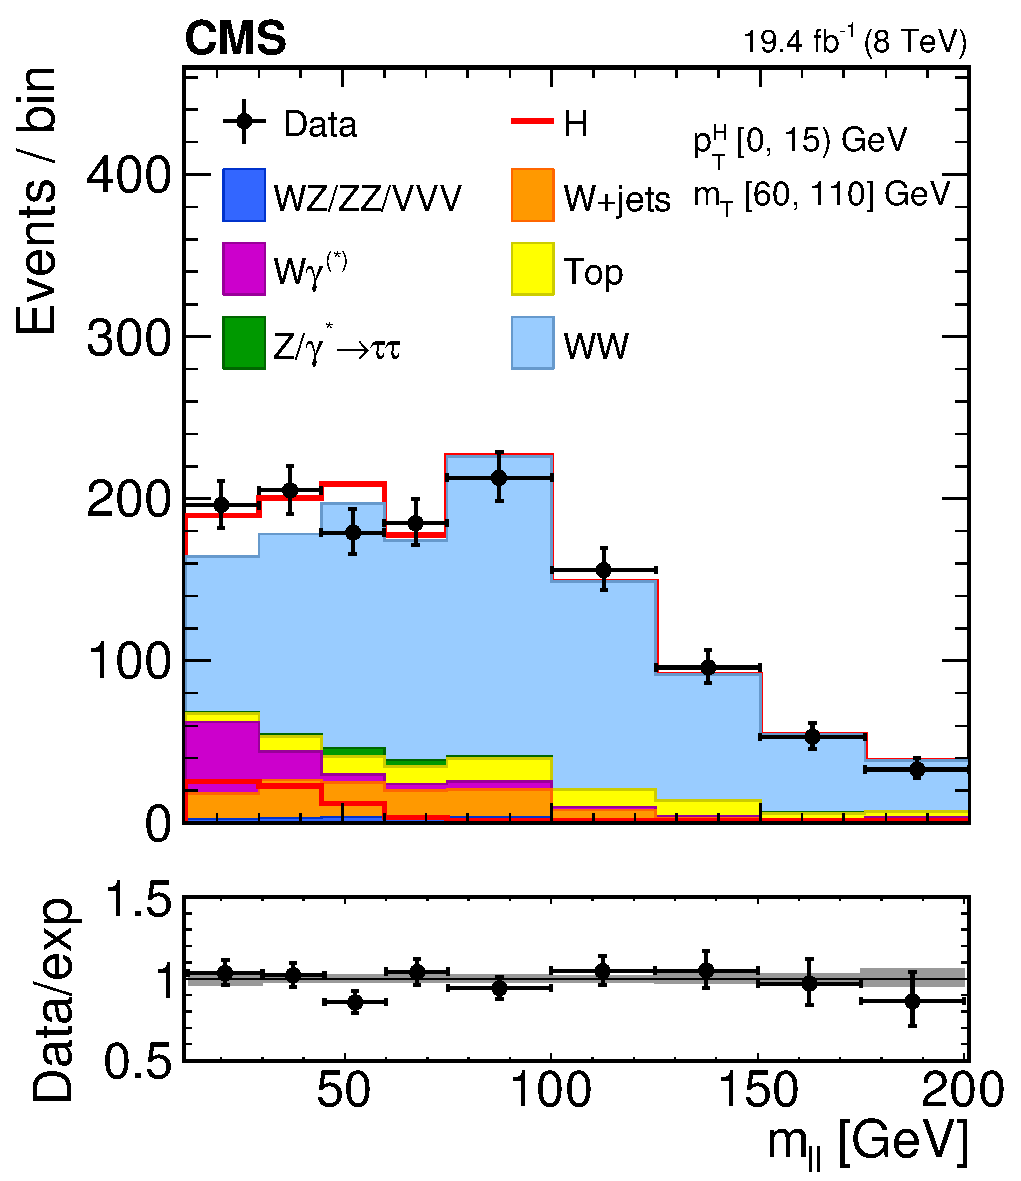
\includegraphics[width=0.3\textwidth]{images/unblinding/mllBin0.pdf}
}
\subfigure{
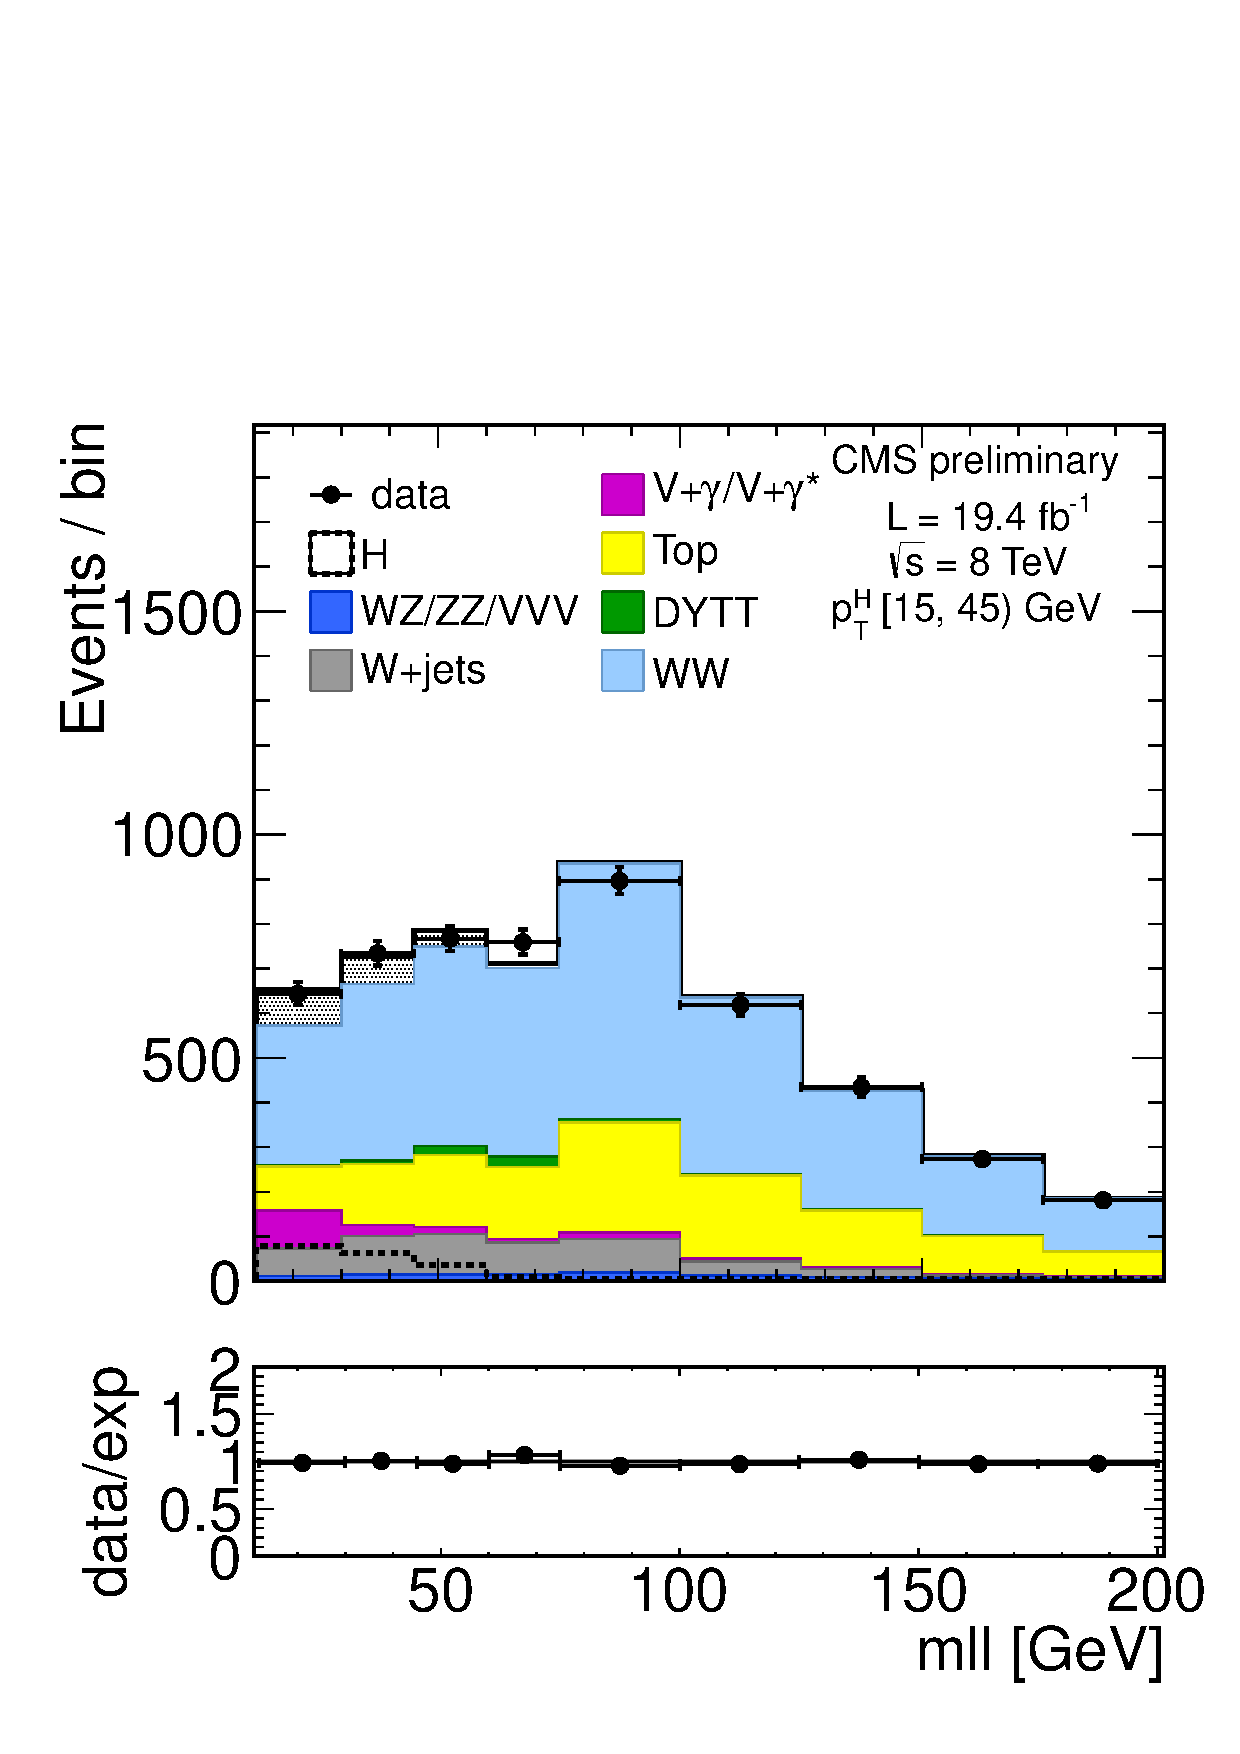
\includegraphics[width=0.3\textwidth]{images/unblinding/mllBin1.pdf}
}
\subfigure{
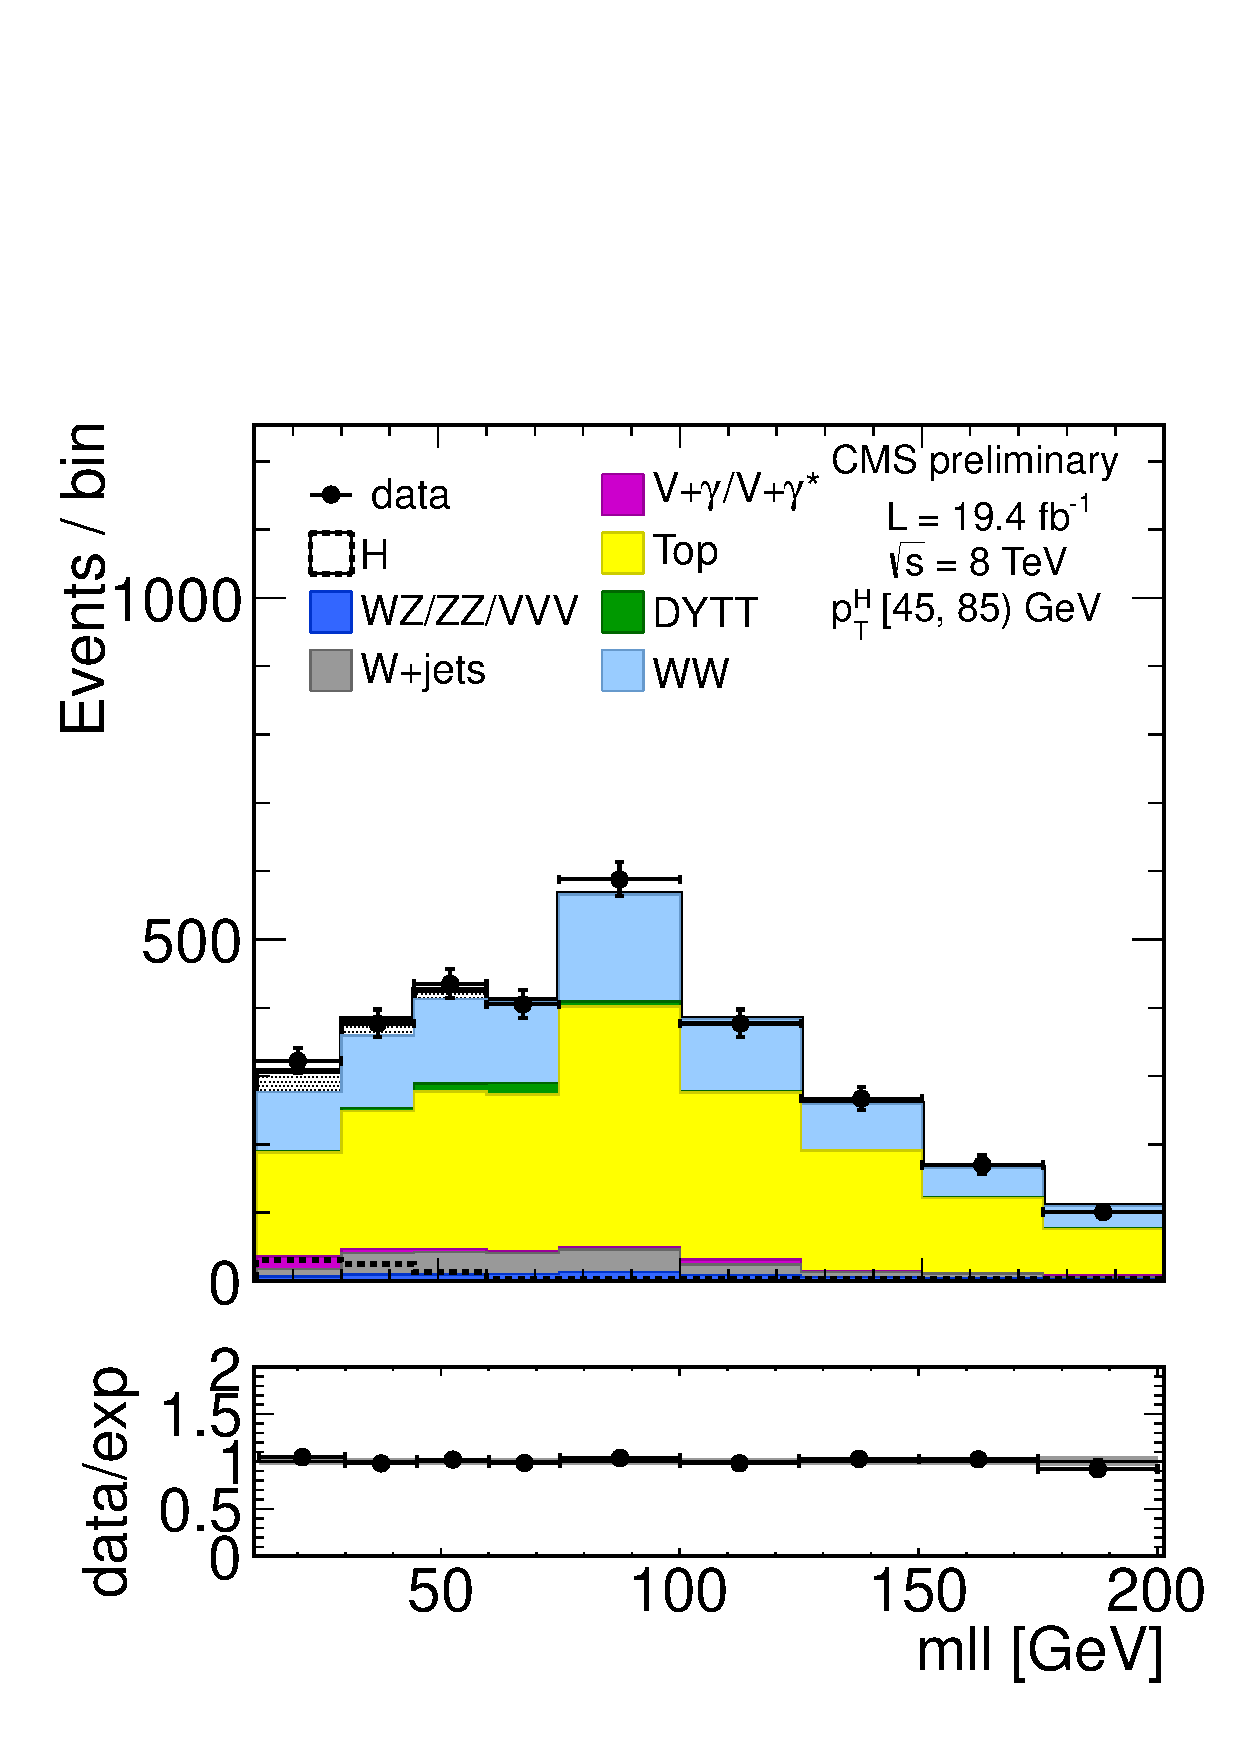
\includegraphics[width=0.3\textwidth]{images/unblinding/mllBin2.pdf}
}\\
\subfigure{
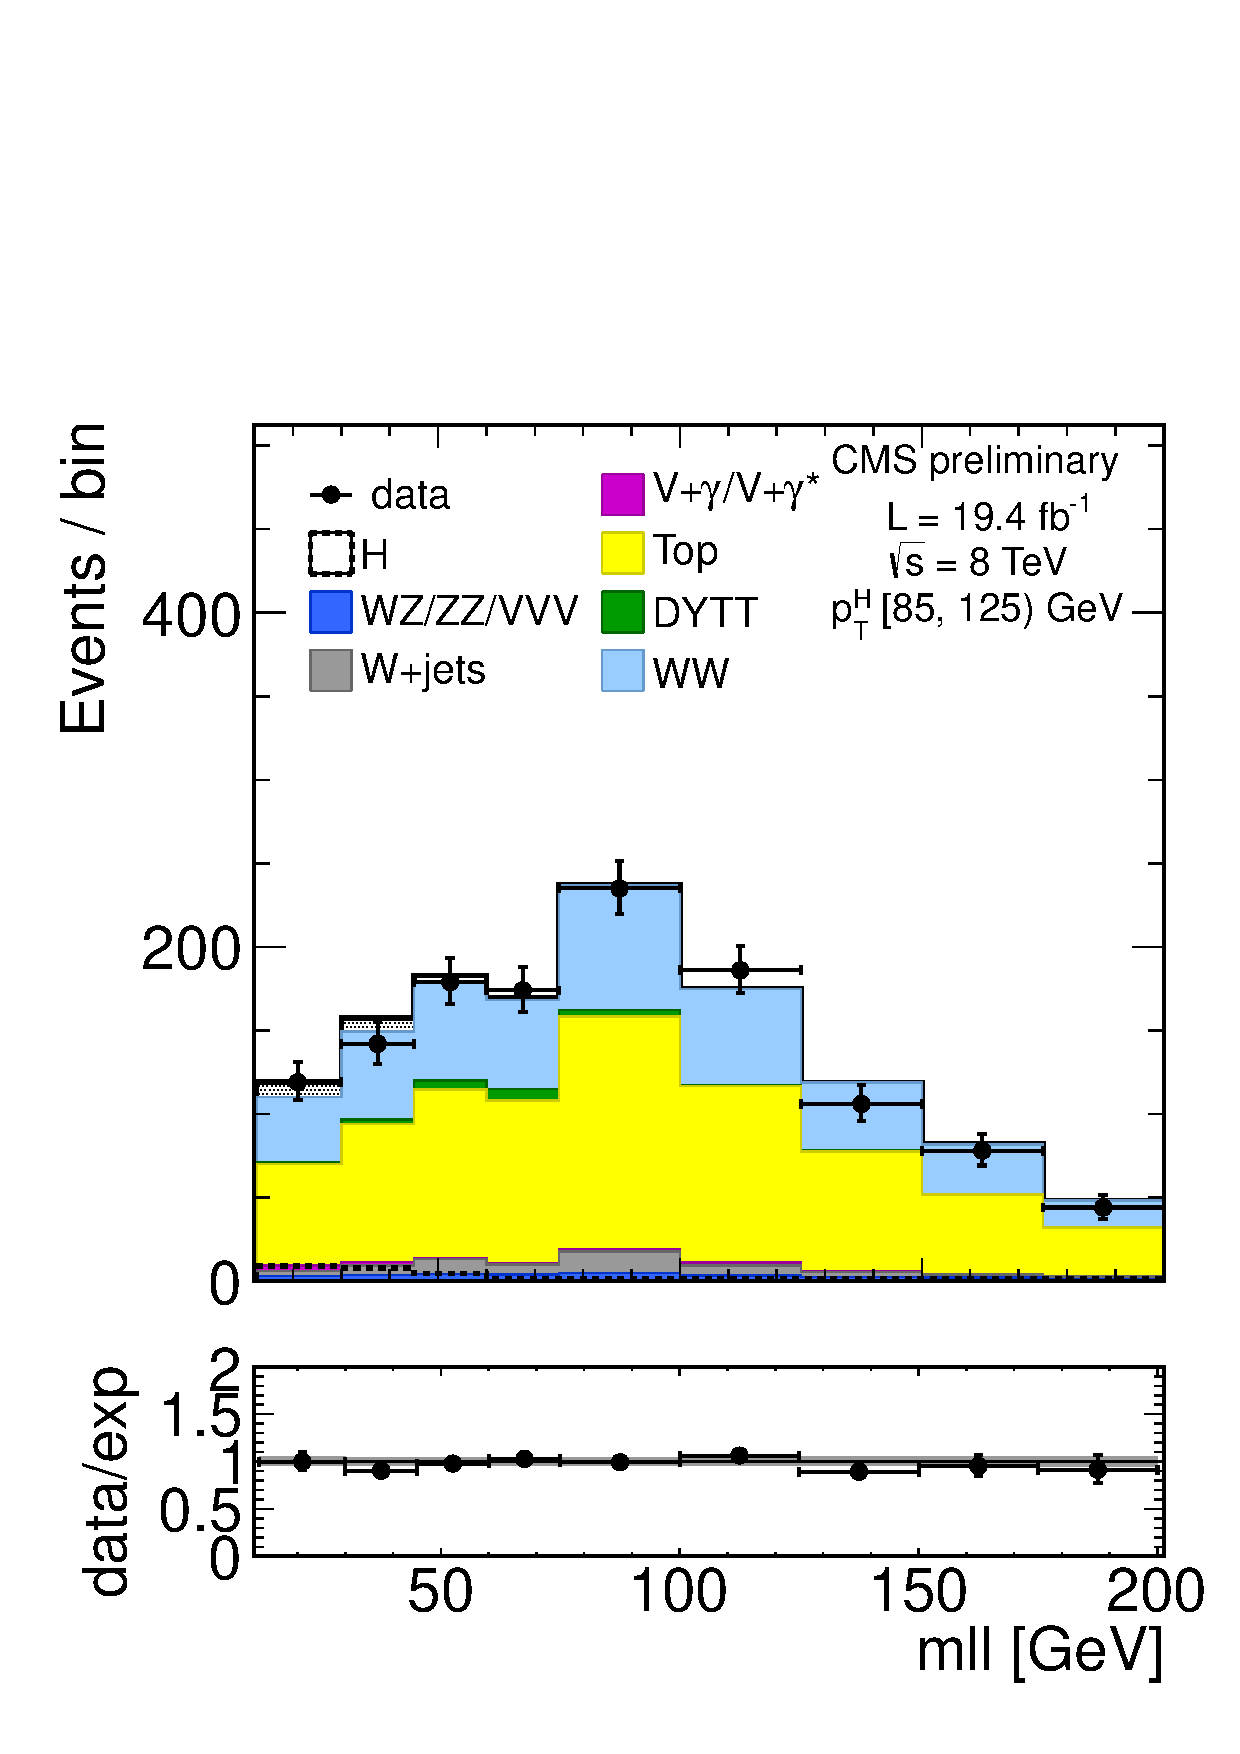
\includegraphics[width=0.3\textwidth]{images/unblinding/mllBin3.pdf}
}
\subfigure{
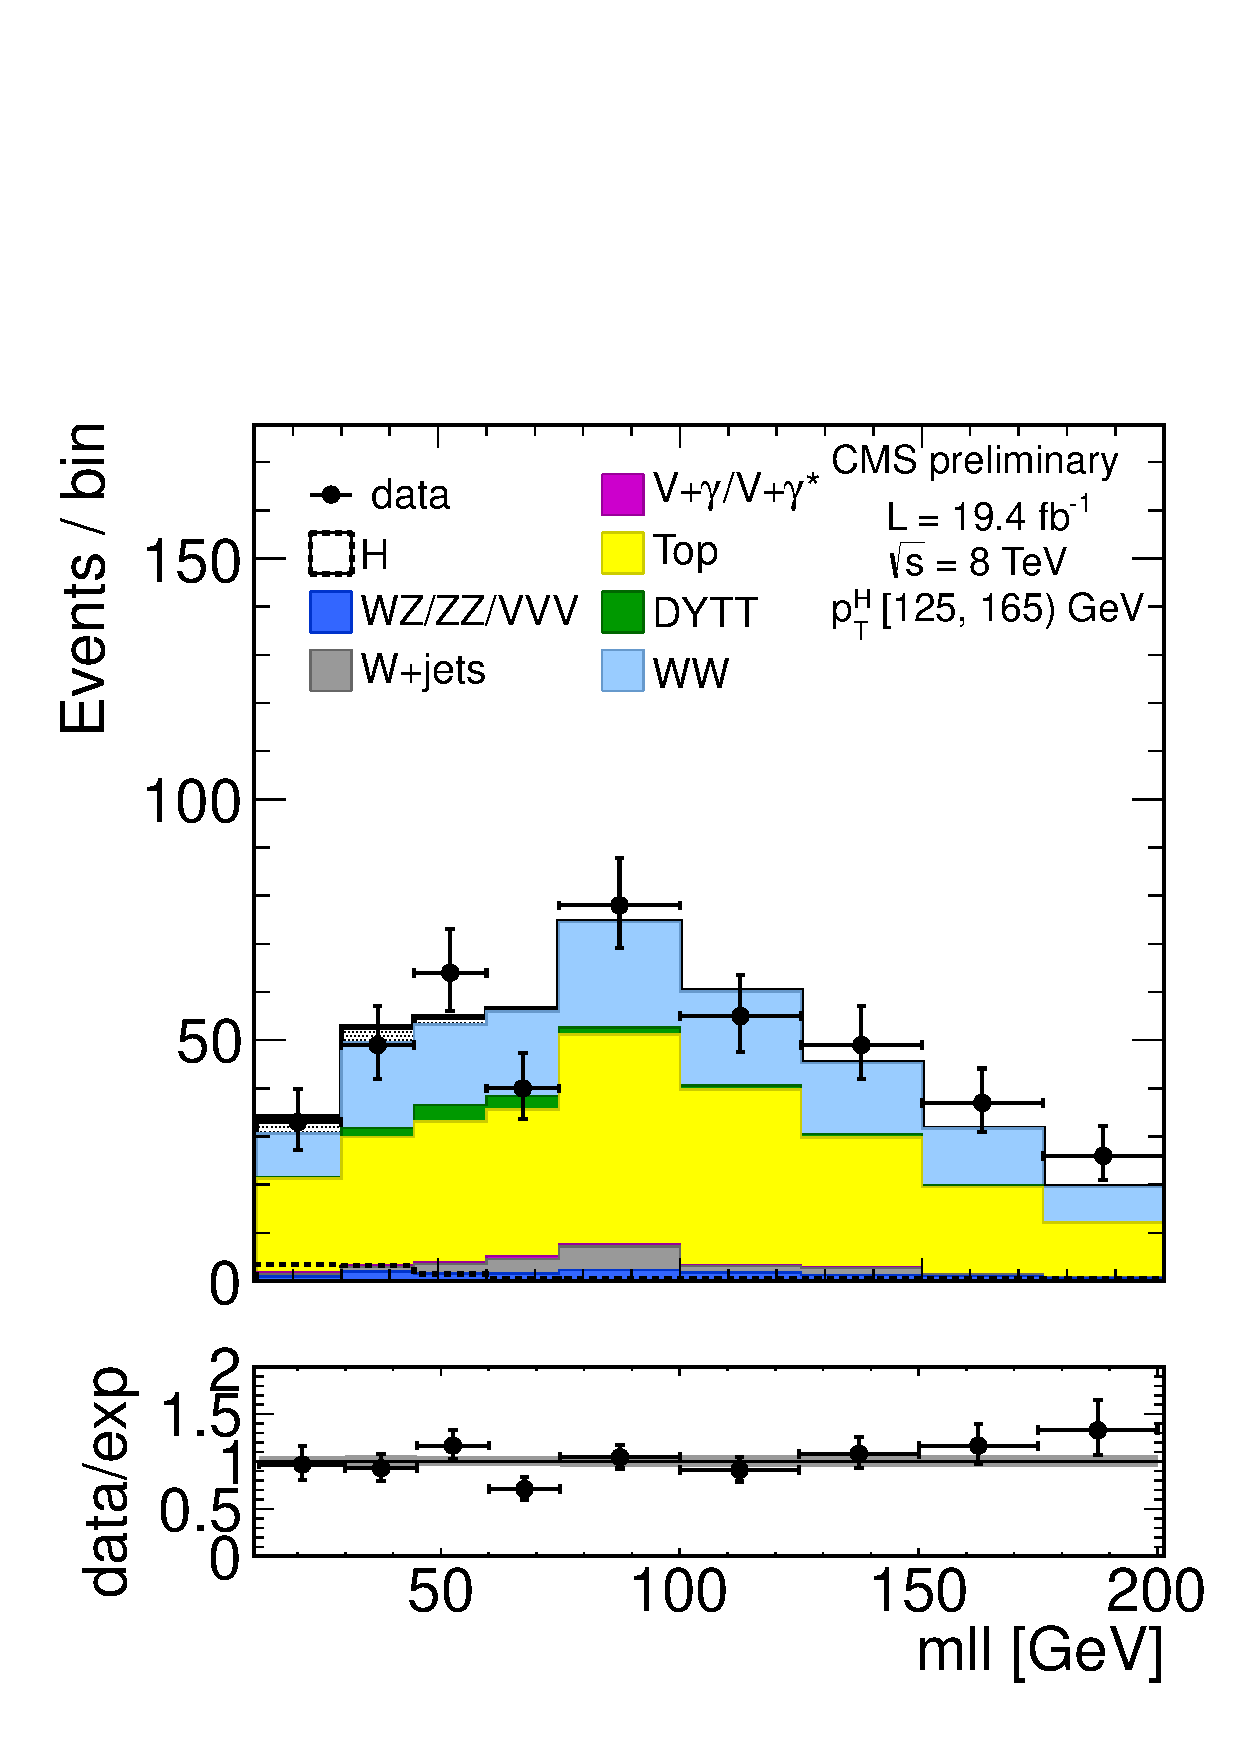
\includegraphics[width=0.3\textwidth]{images/unblinding/mllBin4.pdf}
}
\subfigure{
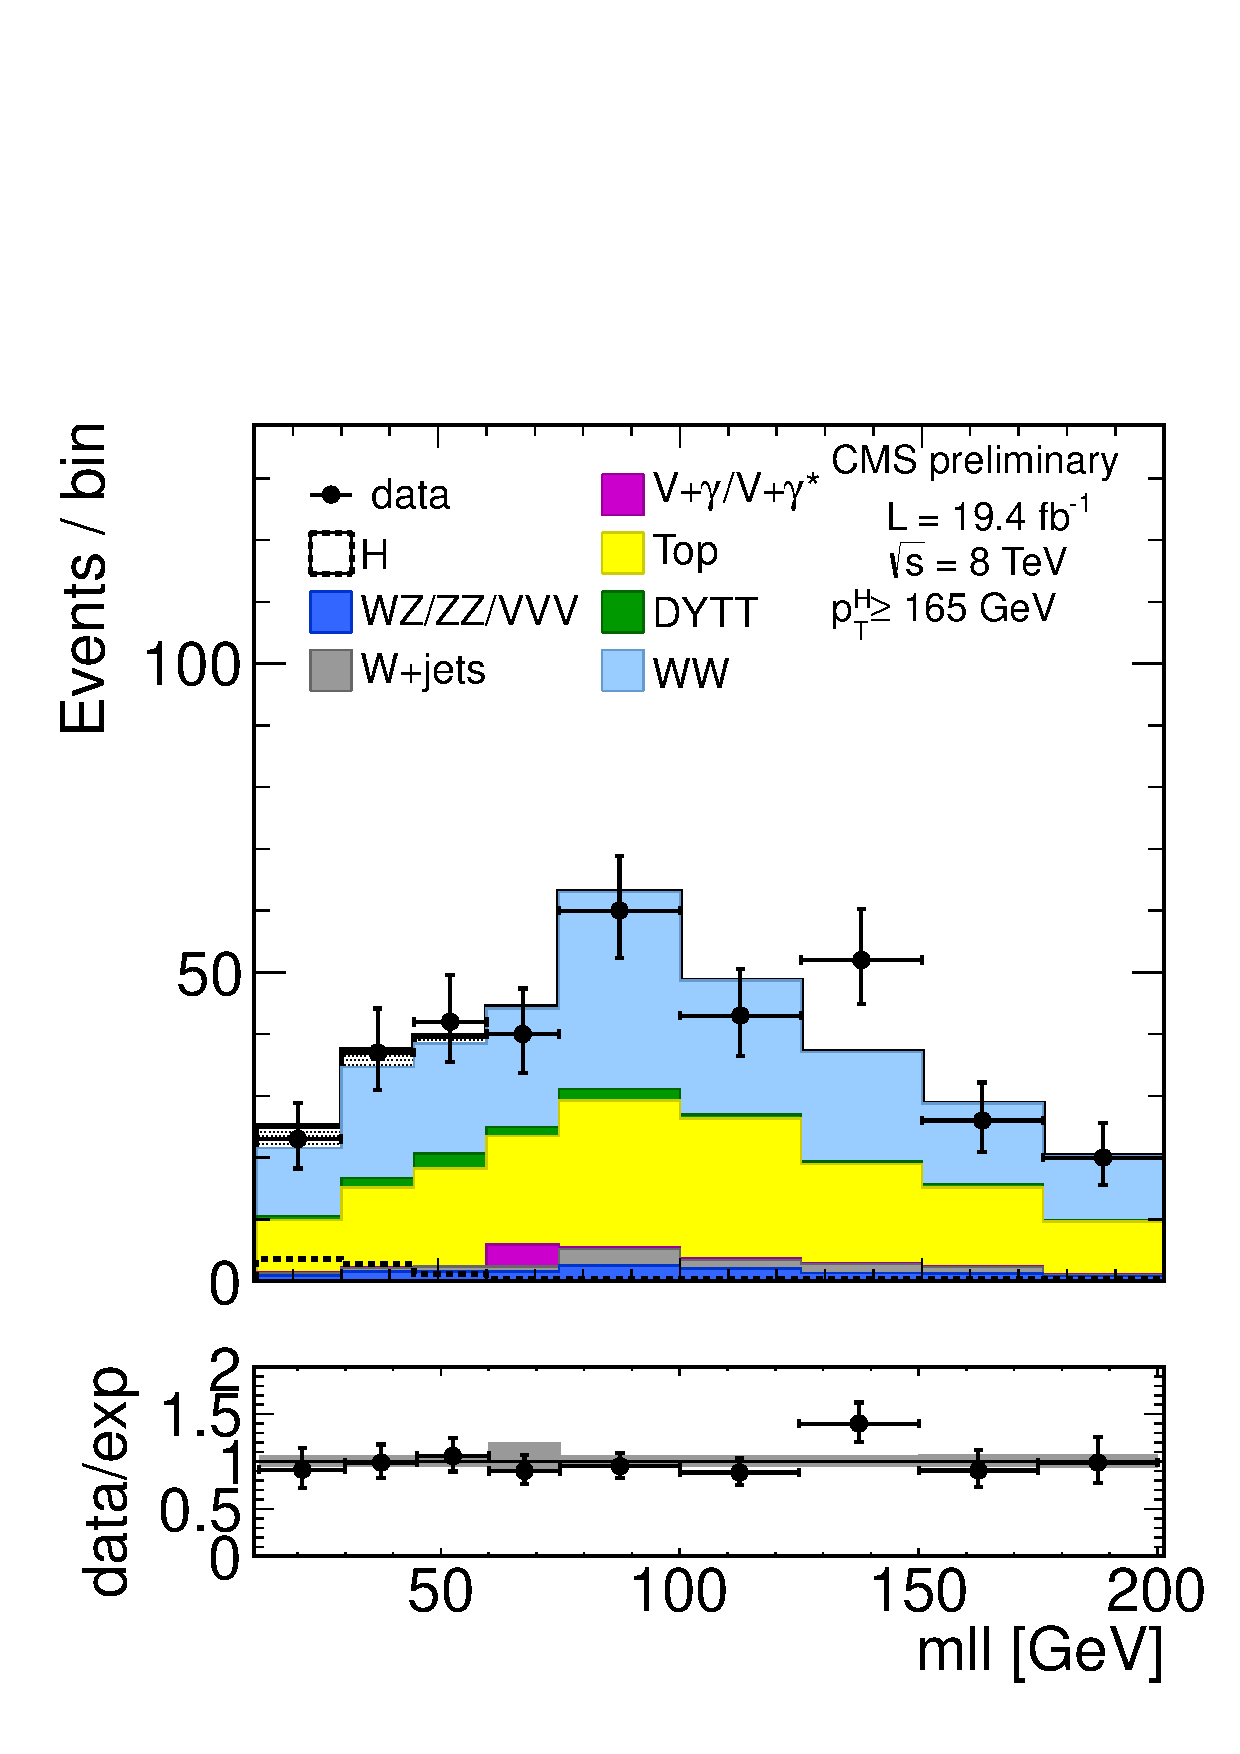
\includegraphics[width=0.3\textwidth]{images/unblinding/mllBin5.pdf}
}
\caption{Distributions of the \mll variable in each of the six \pth bins. Background normalizations correspond to the values obtained from the fit. Signal normalization is fixed to the SM expectation. The distributions are shown in an \mt window of [60,110]\GeV in order to emphasize the Higgs boson (H) signal. The signal contribution is shown both stacked on top of the background and superimposed on it. Ratios of the expected and observed event yields in individual bins are shown in the panels below the plots. The uncertainty band shown in the ratio plot corresponds to the envelope of systematic uncertainties after performing the fit to the data.}\label{fig:mllSignalRegion}
\end{figure}

\begin{figure}[htbp]
\centering
\subfigure{
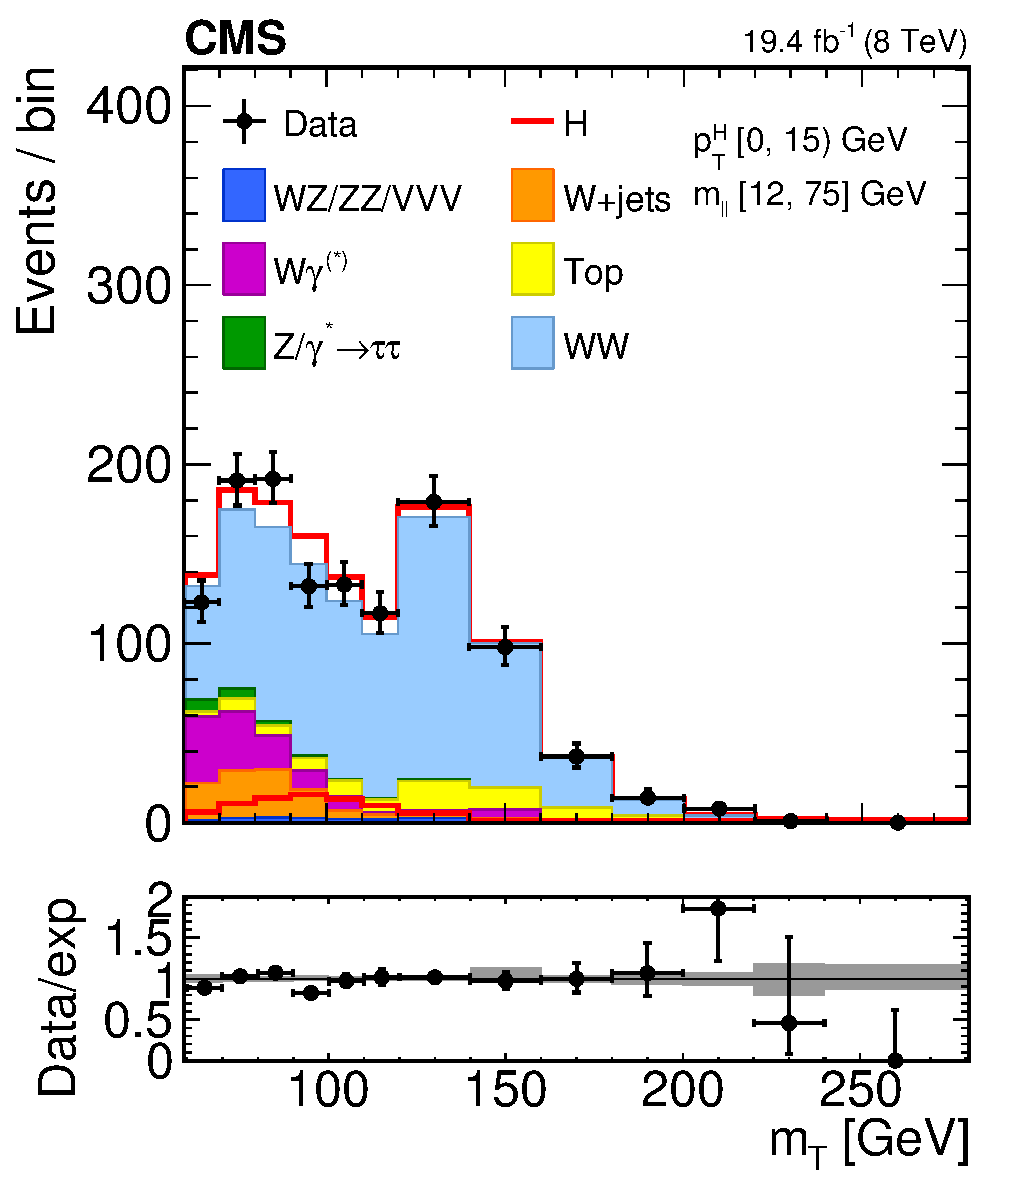
\includegraphics[width=0.3\textwidth]{images/unblinding/mTBin0.pdf}
}
\subfigure{
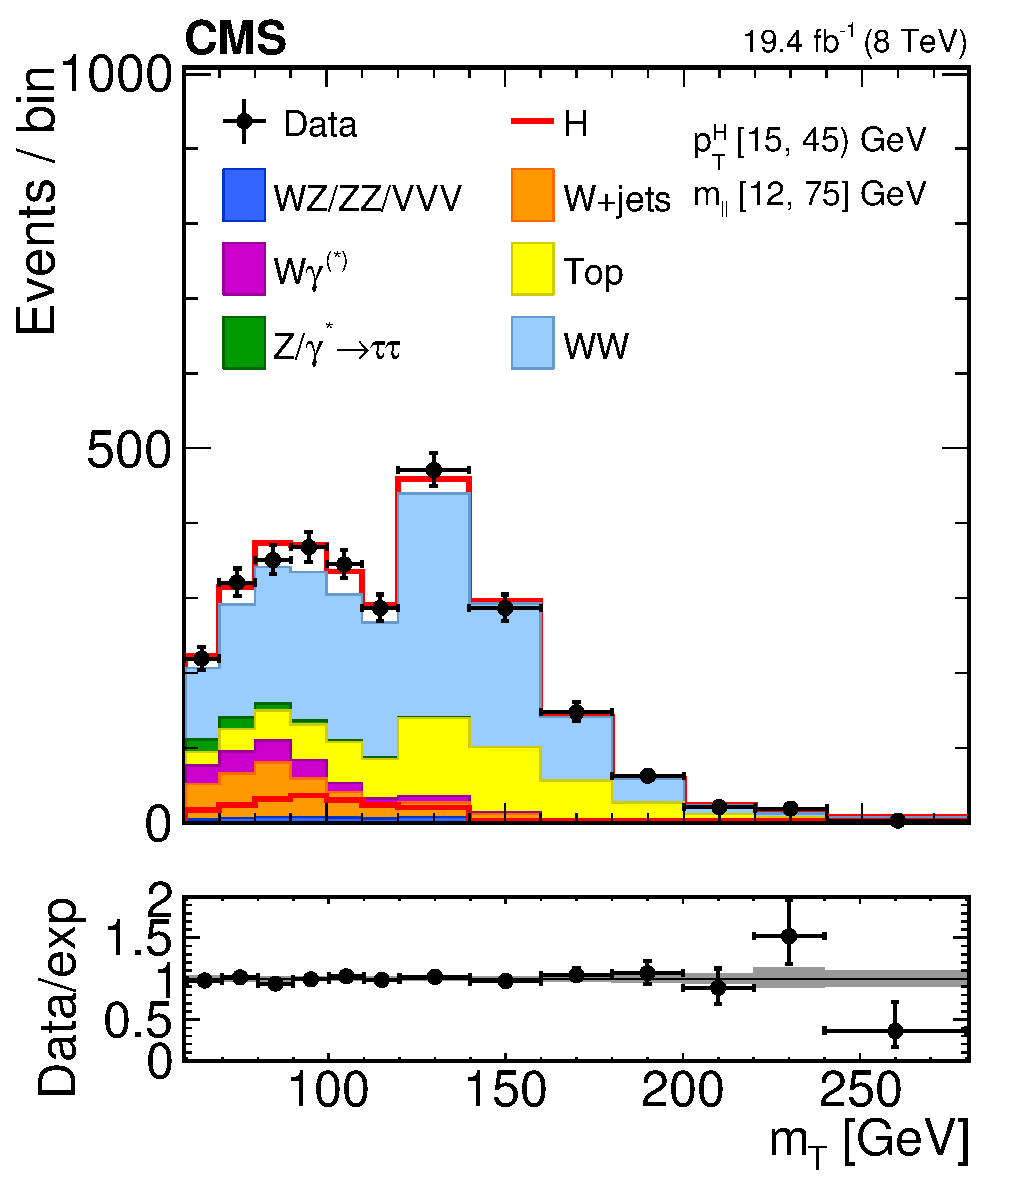
\includegraphics[width=0.3\textwidth]{images/unblinding/mTBin1.pdf}
}
\subfigure{
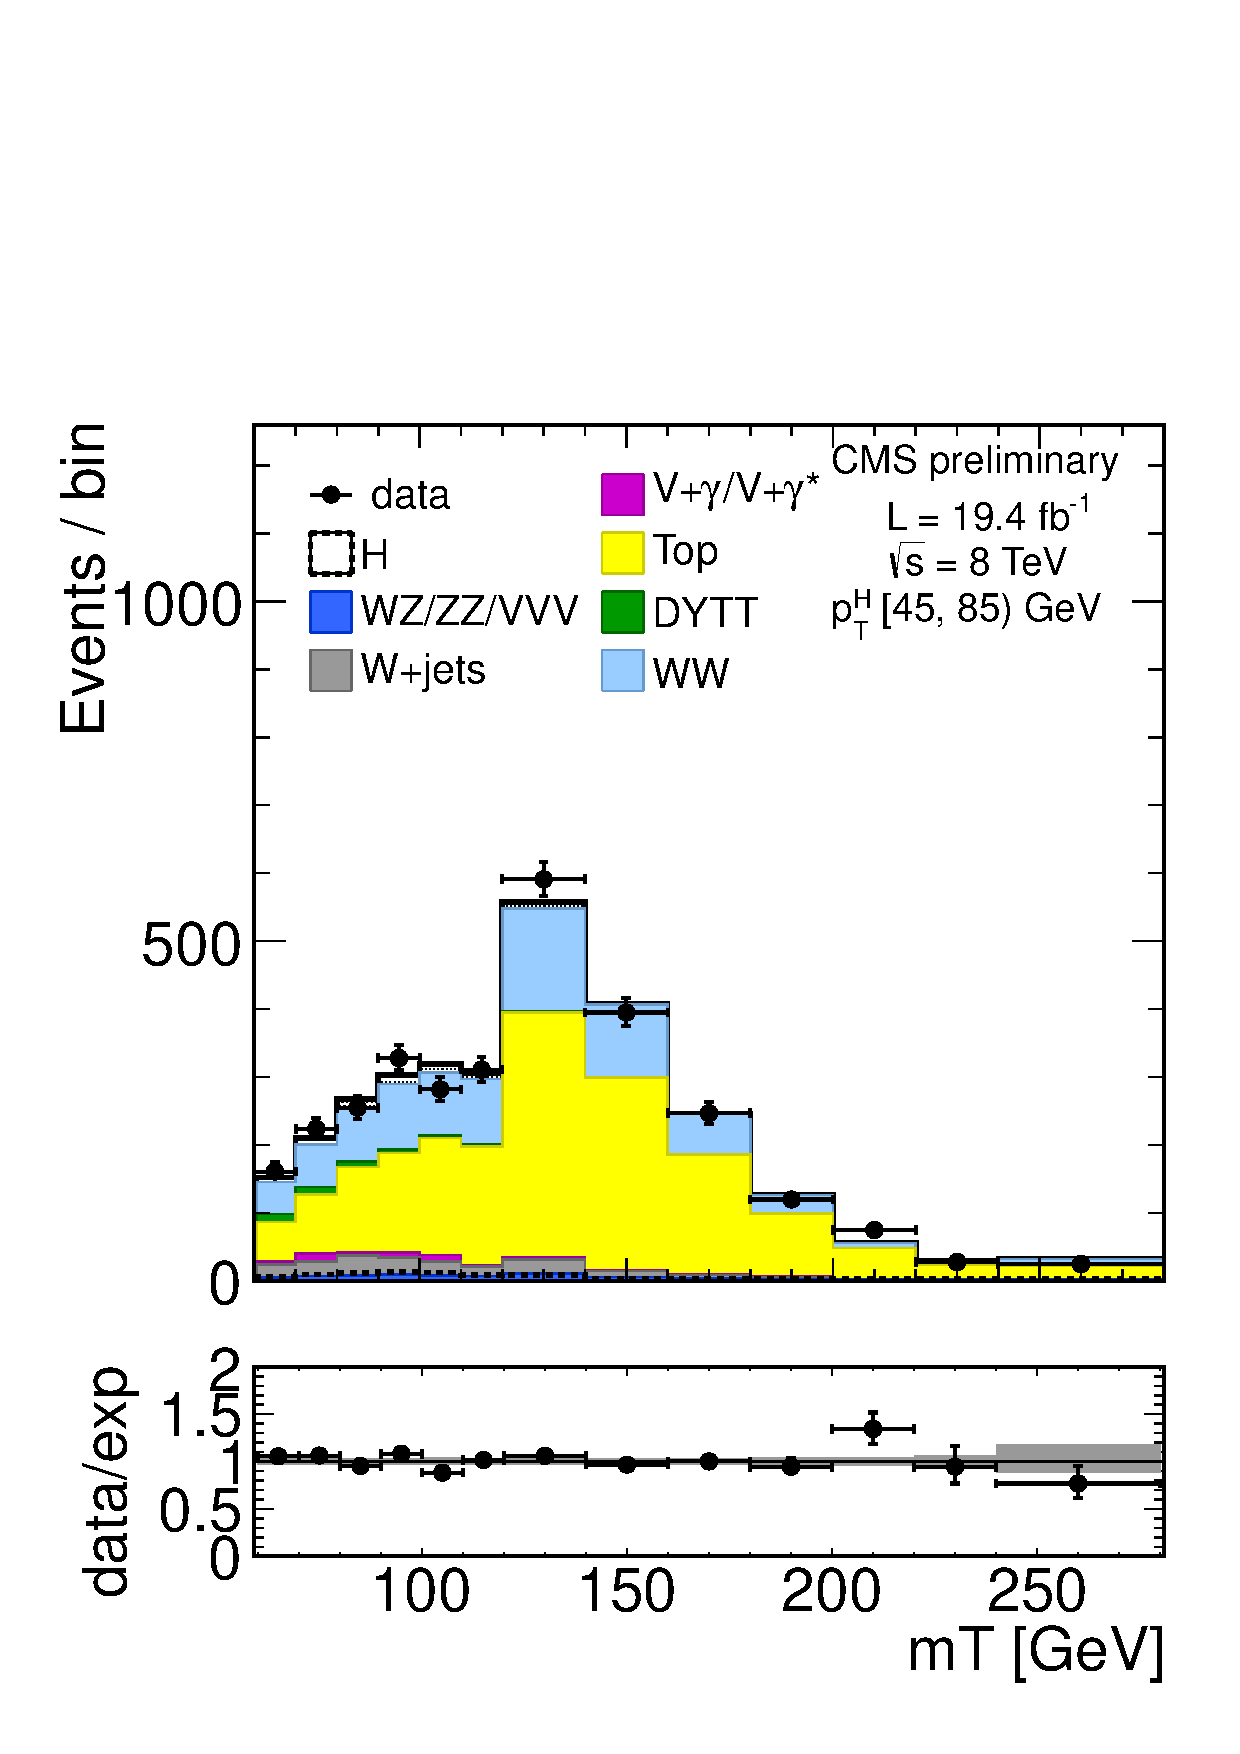
\includegraphics[width=0.3\textwidth]{images/unblinding/mTBin2.pdf}
}\\
\subfigure{
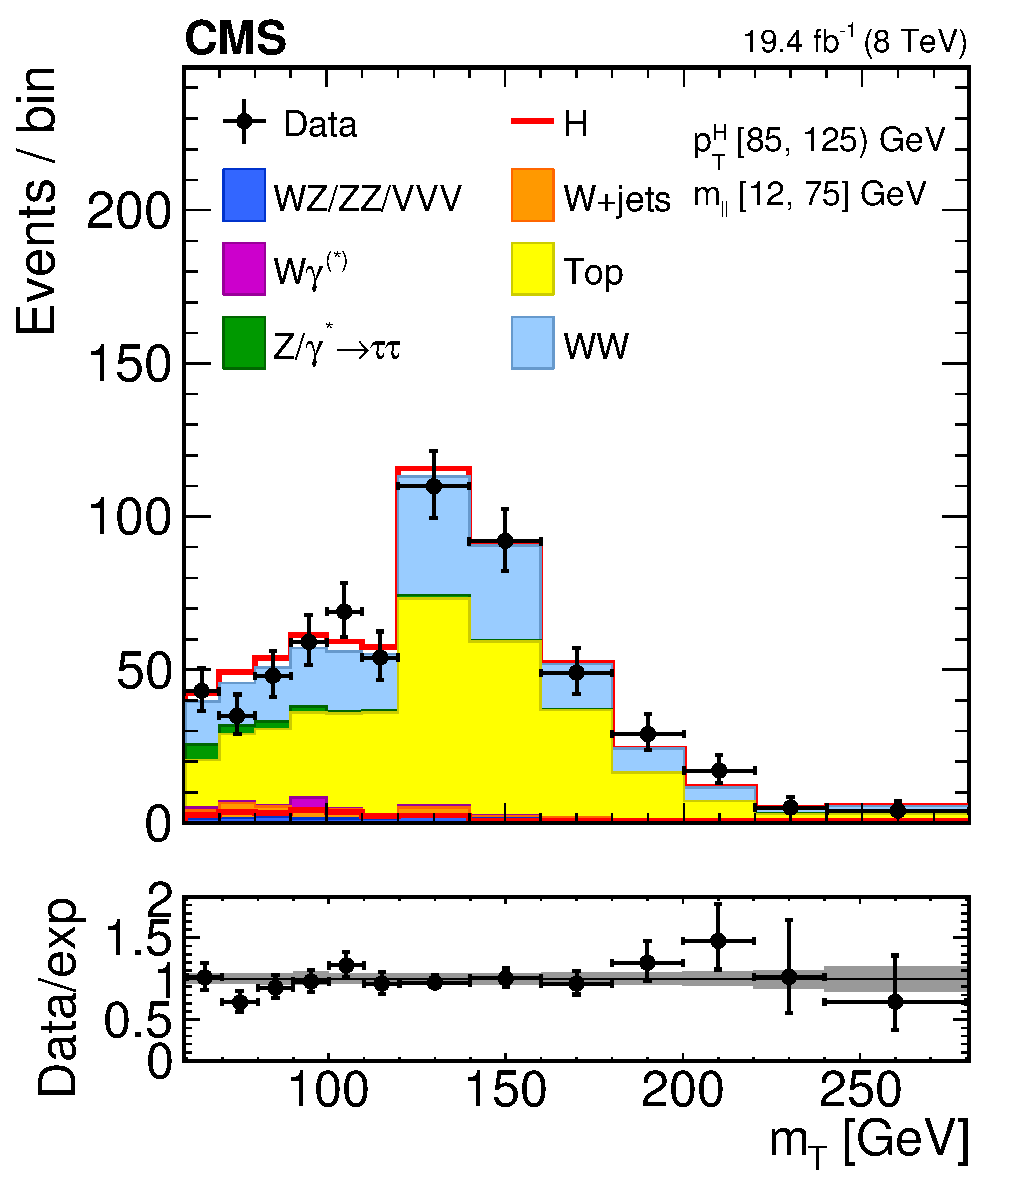
\includegraphics[width=0.3\textwidth]{images/unblinding/mTBin3.pdf}
}
\subfigure{
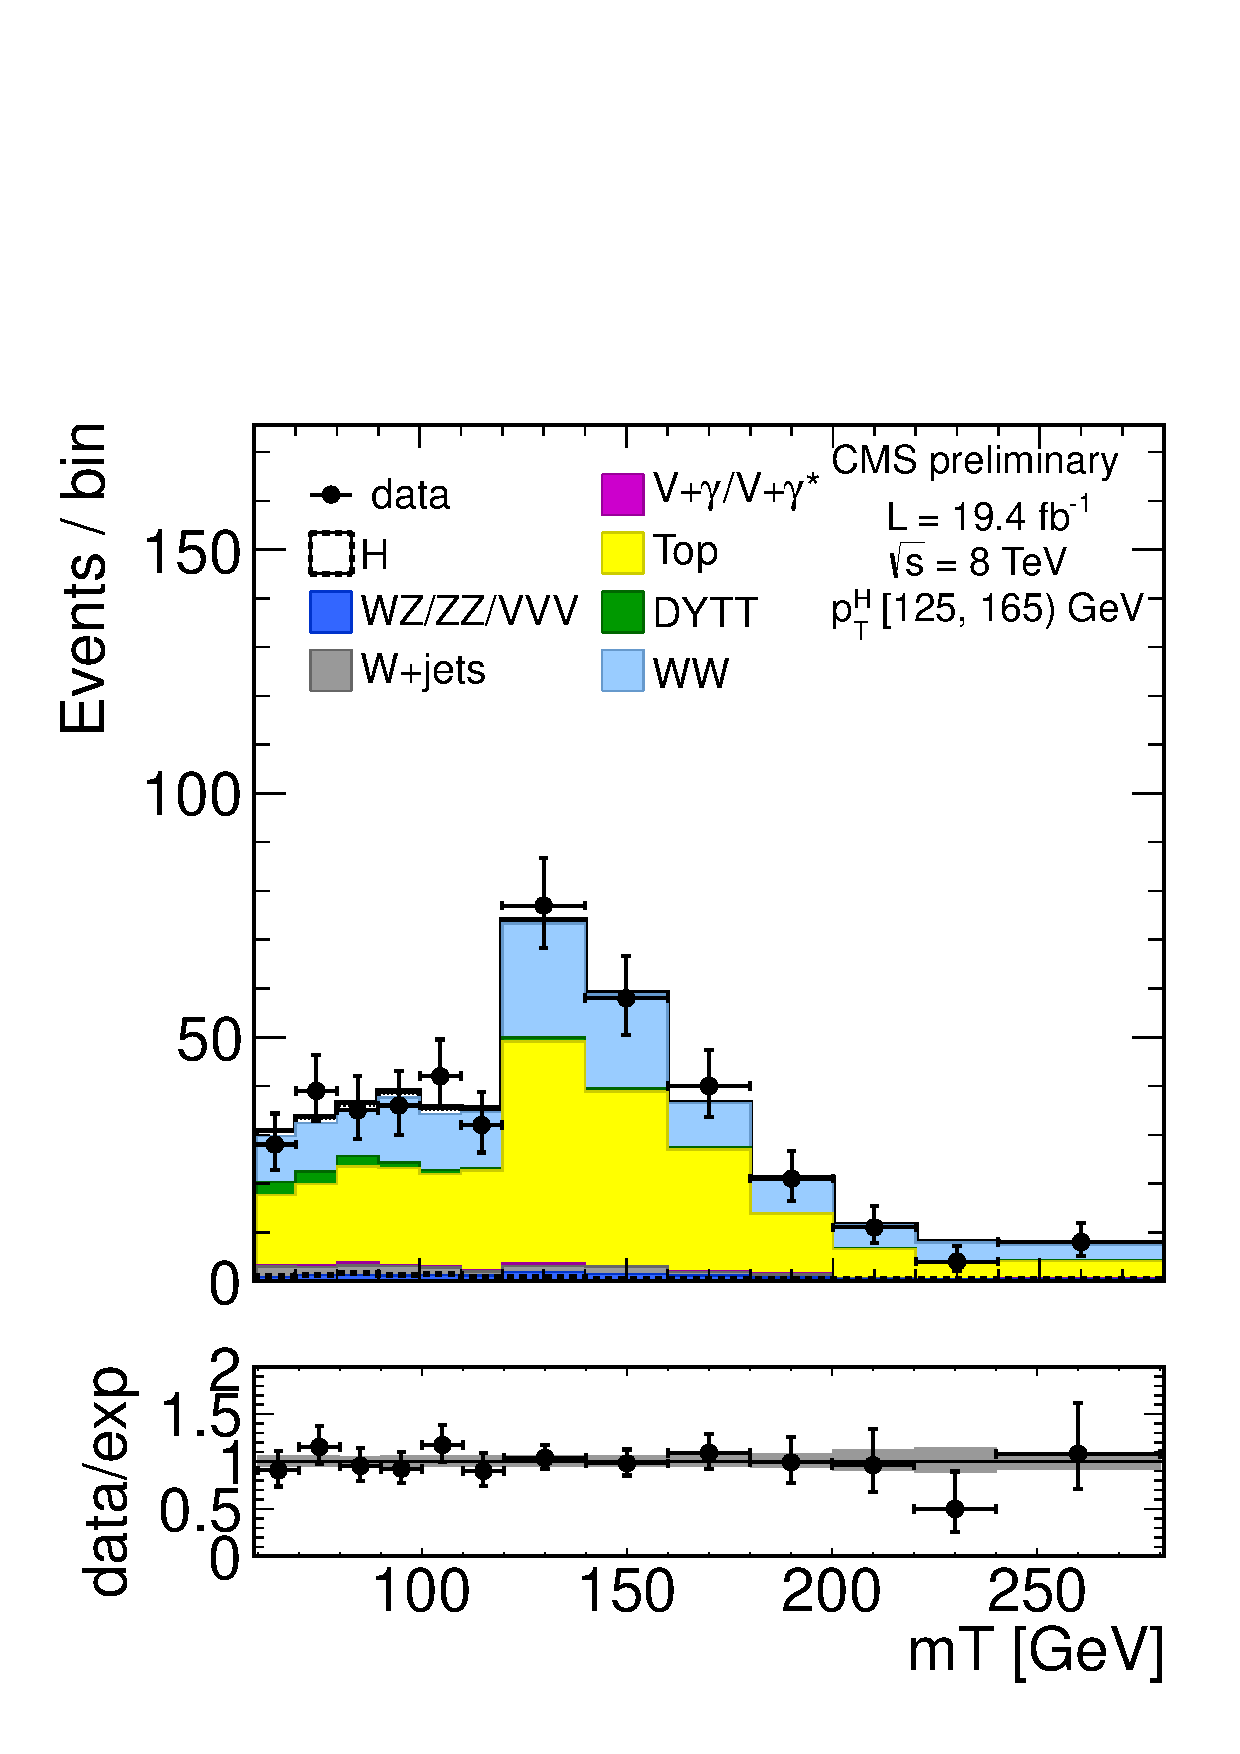
\includegraphics[width=0.3\textwidth]{images/unblinding/mTBin4.pdf}
}
\subfigure{
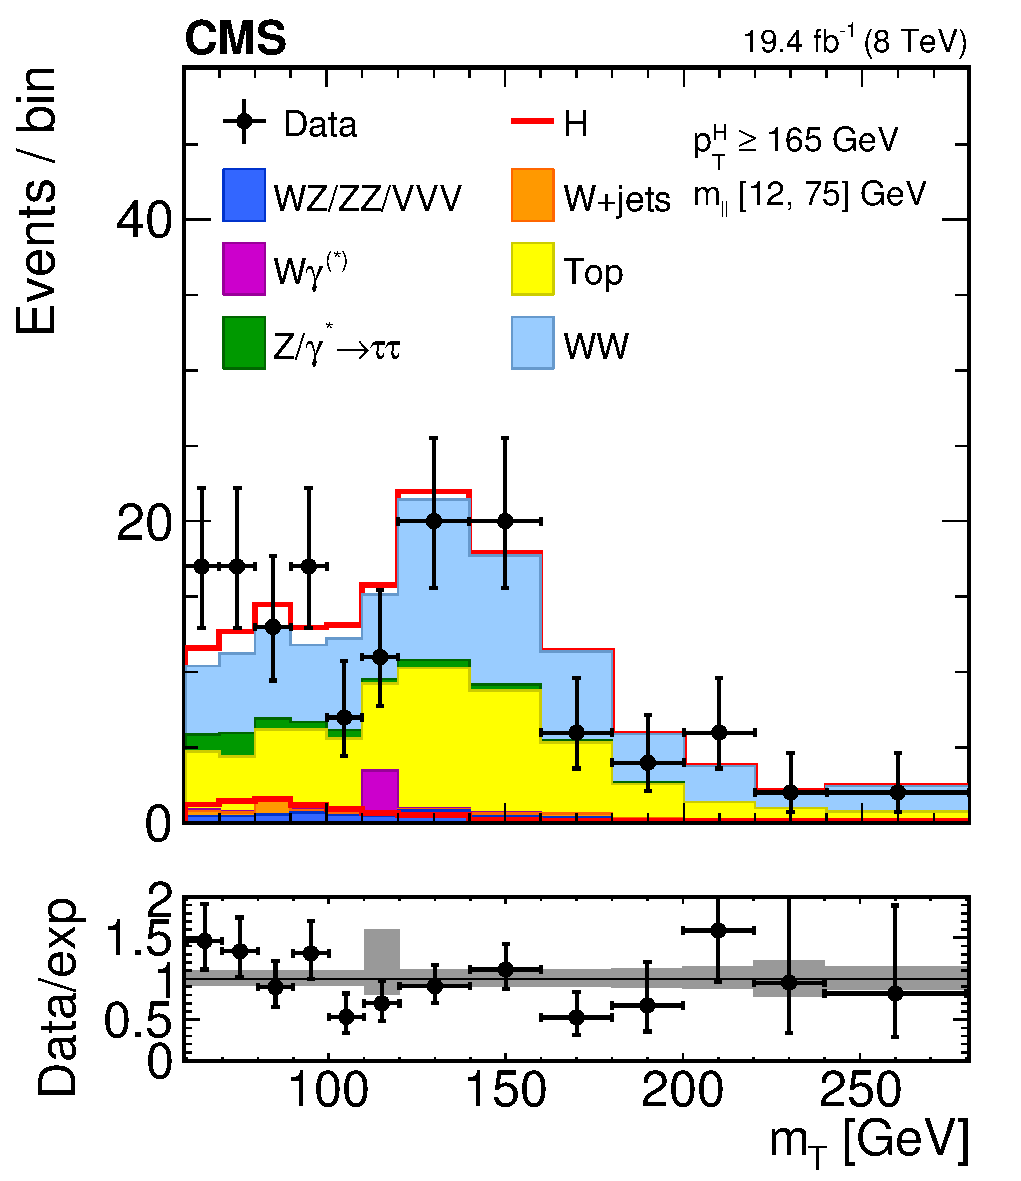
\includegraphics[width=0.3\textwidth]{images/unblinding/mTBin5.pdf}
}
\caption{Distributions of the \mt variable in each of the six \pth{} bins. Background normalizations correspond to the values obtained from the fit. Signal normalization is fixed to the SM expectation. The distributions are shown in an \mll window of [12,75]\GeV in order to emphasize the Higgs boson (H) signal. The signal contribution is shown both stacked on top of the background and superimposed on it. Ratios of the expected and observed event yields in individual bins are shown in the panels below the plots. The uncertainty band shown in the ratio plot corresponds to the envelope of systematic uncertainties after performing the fit to the data.}\label{fig:mTSignalRegion}
\end{figure}

\begin{table}[htb]
\footnotesize{
\begin{center}{
  \caption{Signal prediction, background estimates and observed number of events in data are shown in each \pth{} bin after applying the analysis selection requirements. The total uncertainty on the number of events is reported. For signal processes, the yield related to the ggH are shown, separated with respect to the contribution of the other production mechanisms (XH=VBF+VH). The WW process includes both quark and gluon induced contribution, while the Top process takes into account both \ttbar and tW. }\label{table:yields}
\begin{tabularx}{\textwidth}{ l >{\centering}X >{\centering}X >{\centering}X >{\centering}X >{\centering}X >{\centering}X }

\toprule

\multirow{2}{*}{Process} & \multicolumn{6}{c}{\pth [\GeV]} \tabularnewline
 &	0--15	&	15--45	&	45--85	&	85--125	&	125--165	&	165--$\infty$ \tabularnewline

\midrule

ggH	&	$73\pm3$	&	$175\pm5$	&                $59\pm3$	&                $15\pm2$	&                $5.1\pm1.5$	&                $4.9\pm1.4$	\tabularnewline
XH=VBF+VH	&	$4\pm2$ 	&	$15\pm4$ 	&		 $16\pm4$	&	         $8\pm2$ 	&		 $3.8\pm1.1$ 	&		 $3.0\pm0.8$    \tabularnewline
Out-of-fiducial & $9.2\pm0.5$   &       $19.9\pm0.7$    &      $11.4\pm0.6$    &    $4.4\pm0.3$   &     $1.6\pm0.2$   &   $2.4\pm0.2$ \tabularnewline
Data 	&	2182	 	&         5305	 	&	         3042	 	& 	          1263	 	&	         431	 	& 	          343	 	\tabularnewline
Total background &  	 $2124\pm128$	 &     $5170\pm321$	 &       $2947\pm293$	 &            $1266\pm175$	 &         $420\pm80$	 &              $336\pm74$	 \tabularnewline

WW 	& 		$1616\pm107$	 &	 $3172\pm249$	 &	     $865\pm217$	 &	     $421\pm120$	 &	     $125\pm60$	 &		     $161\pm54$	 \tabularnewline
Top 	&	$184\pm38$	&	                $1199\pm165$	&	                $1741\pm192$	&	                $735\pm125$	&	                $243\pm51$	& 	        $139\pm49$	\tabularnewline
W+jets 	& $134\pm5$ 	&	         $455\pm10$ 	&	         $174\pm6$ 	&	         $48\pm4$ 	&	         $14\pm3$ 	&	         $9\pm3$ 	\tabularnewline
WZ+ZZ+VVV & $34\pm4$ 	 &	$107\pm10$ 	&                $71\pm7$ 	&	         $29\pm5$ 	&                $14\pm3$ 	&     $13\pm4$ 	\tabularnewline
\dytt 	&	$23\pm3$ 	&         $67\pm5$ 	&         $47\pm4$ 	&         $22\pm3$ 	&         $12\pm2$ 	&         $10\pm2$ 	\tabularnewline
W$\gamma^{(*)}$	& $132\pm49$     &             $170\pm58$    &              $48\pm30$ &                  $12\pm9$ &                  $3\pm3$ &                 $5\pm10$ \tabularnewline

\bottomrule

  \end{tabularx}
  }
   
  \end{center}
  }
\end{table}

The signal strengths obtained performing the fit are shown in Table~\ref{tab:signal_strengths}.
In order to assess the robustness of the fit, several toy MC samples have been generated with a mean value for each bin corresponding to the sum of the expected background plus signal events and a statistical accuracy comparable to the one expected in data. Each toy sample is fitted with the same procedure described before. The distribution of the signal strengths extracted in each bin using the toy MC samples are found to be consistent with 1, implying that no bias is introduced by the fit procedure. 
%Moreover, the pull distribution of each signal strength has also been checked, showing an average and RMS value consistent with 0 and 1, respectively.

\begin{table}[htb]
\caption{Signal strengths measured in data for each \pth bin with 68$\%$ CL uncertainties.}\label{tab:signal_strengths}
\begin{center}
\begin{tabular}{ c  c  c  } \toprule
 \pth [GeV] & $\mu$  & Uncertainty (68$\%$ CL) \\ \midrule
 0--15   &  +0.753  & -0.424/+0.437  \\
 15--45   &  +0.716  & -0.300/+0.308  \\
 45--85   &  +1.309  & -0.445/+0.465  \\
 85--125   &  +0.165  & -0.890/+0.898  \\
 125--165   &  +1.715  & -1.103/+1.217  \\
 165--$\infty$   &  +0.796  & -0.913/+1.059  \\
 \bottomrule
\end{tabular}
\end{center}
\end{table}

%\begin{figure}[htb]
%\centering
%\subfigure[]{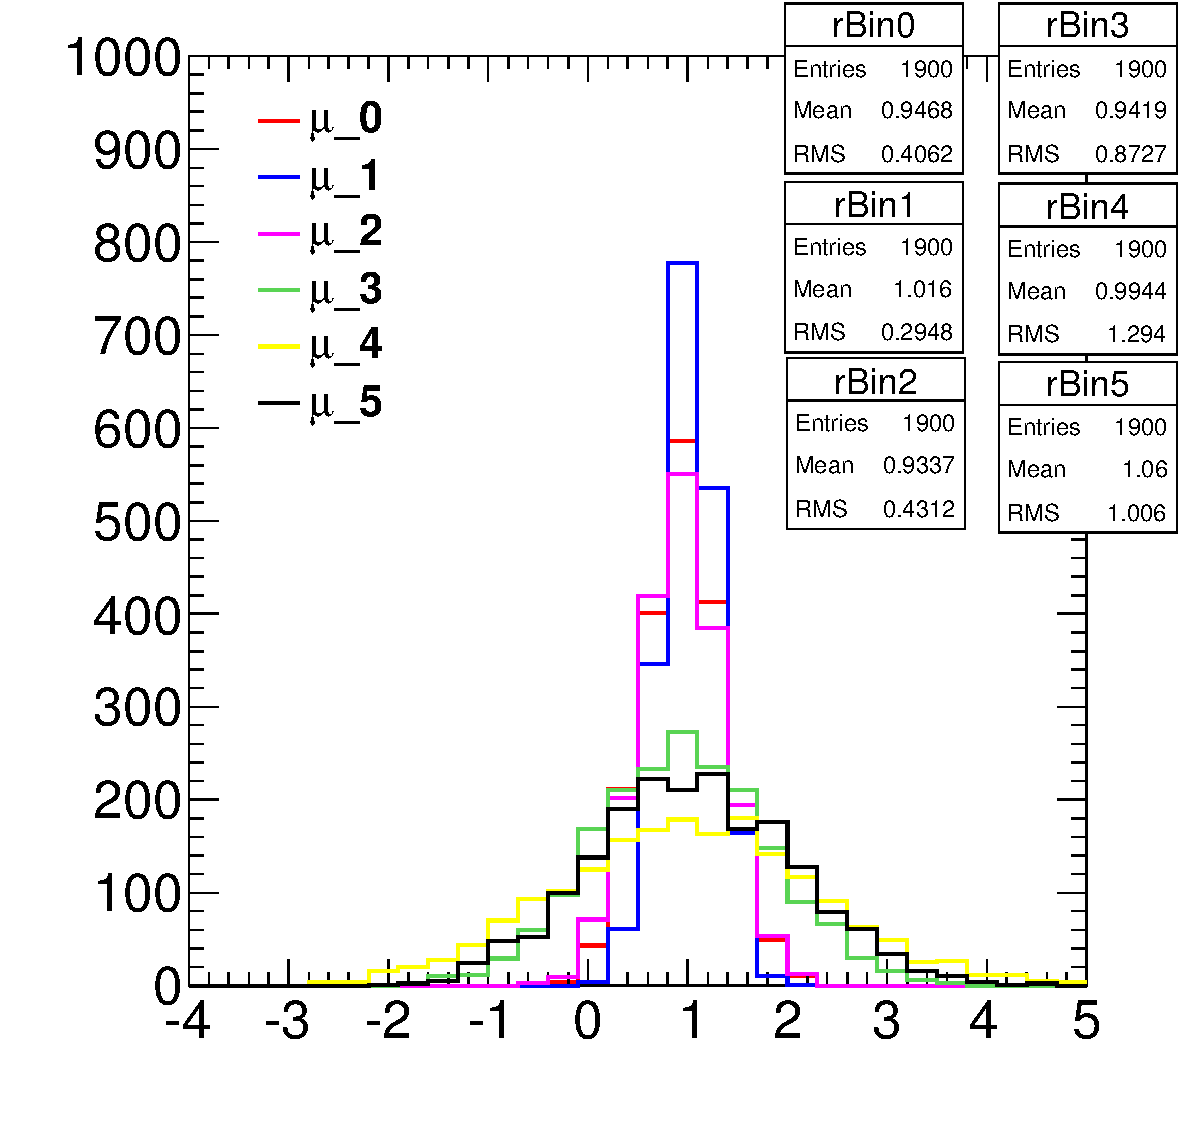
\includegraphics[width=0.45\textwidth]{images/mu_toys.pdf}}
%\subfigure[]{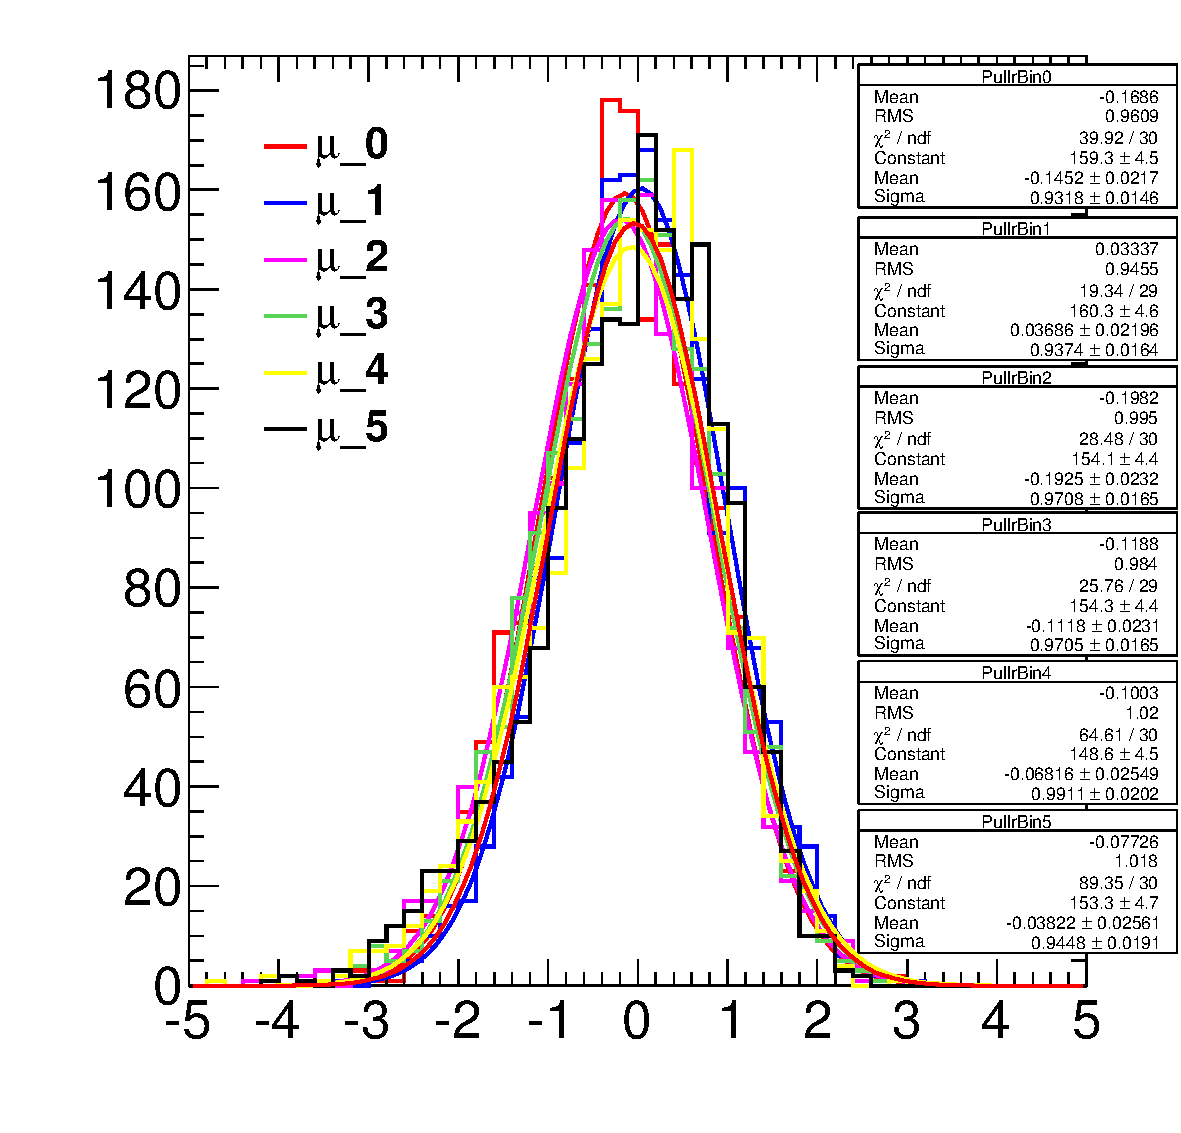
\includegraphics[width=0.45\textwidth]{images/pull_toys.pdf}}
%\caption{Signal strength distribution as extracted from the fit of toy MC samples (a). Distribution of the pull of the signal strength parameters (b).\label{fig:pull_fit}}
%\end{figure}


%The signal yield after the fit with data is found to be of $318 \pm 12$ events, to be compared with the expected value of $382 \pm 7$ events.
The reconstructed spectrum is obtained starting from the signal yield $N_i$ in each \pth bin $i$, obtained subtracting the out-of-fiducial events as shown in Eq.~\eqref{eq:sig_yield}, and dividing it by the bin width $w_i$ and integrated luminosity $\mathcal{L}$, i.e.:
\begin{equation}
\frac{d\sigma_i}{d p_\mathrm{T,reco}^\mathrm{H}} = \frac{N_i}{w_i \mathcal{L}} \quad.
\end{equation}

The spectrum shown in Fig. \ref{fig:pre_unfolding} is obtained after having performed the fit and after the subtraction of the out-of-fiducial signal events, but before undergoing the unfolding procedure. The theoretical distribution after the detector simulation and event reconstruction is also shown for comparison. Also, the expected distribution of the sub-dominant VBF and VH production mechanisms is displayed.

\begin{figure}[htb]
\centering
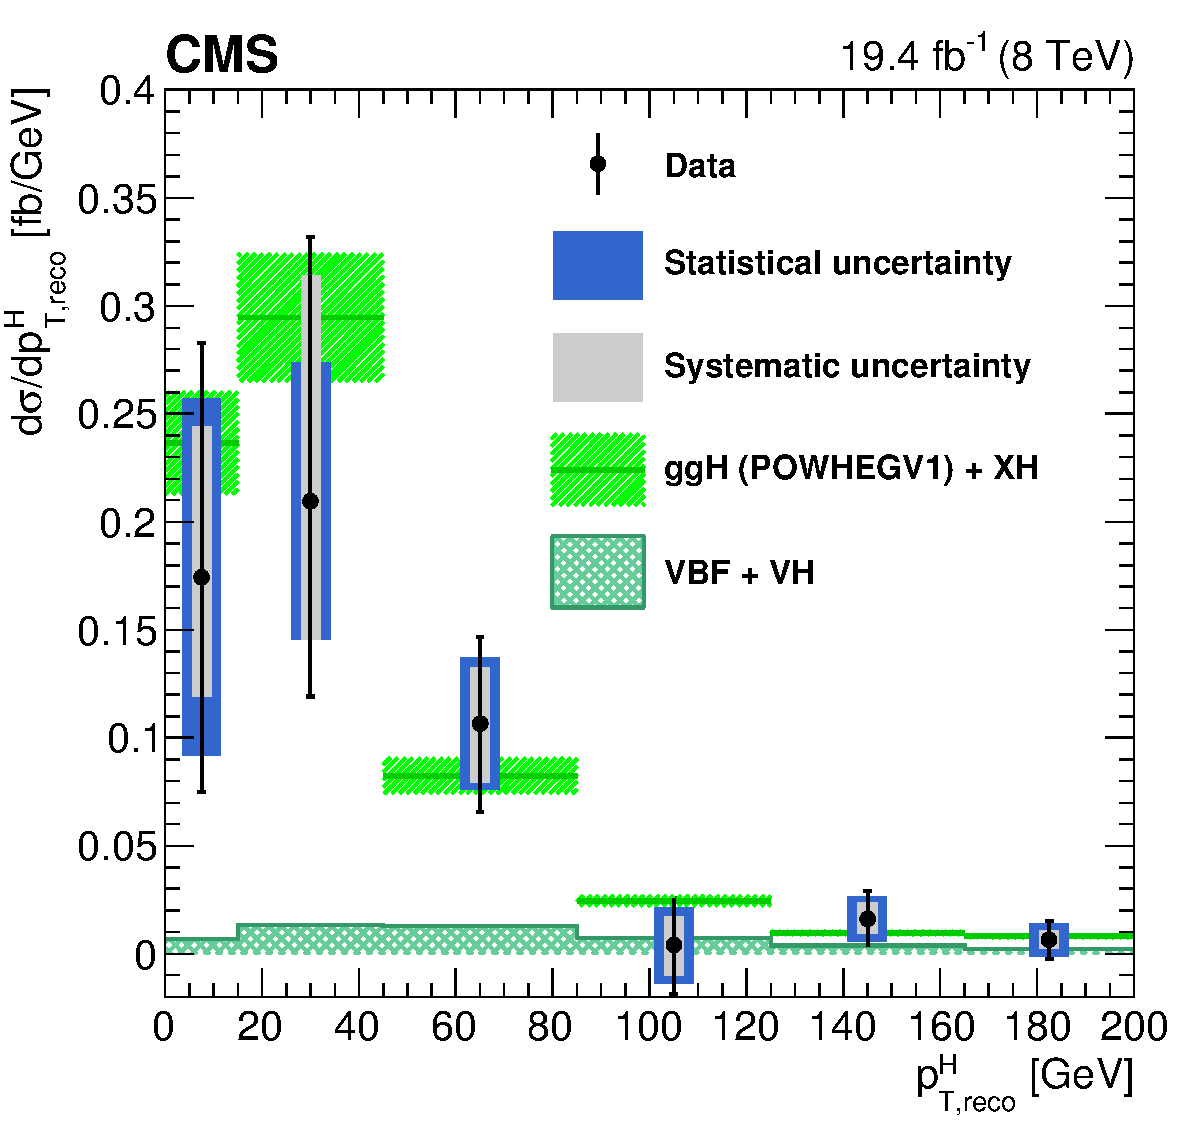
\includegraphics[width=0.7\textwidth]{images/unblinding/pth_reco_paper.pdf}
\caption{Differential Higgs boson production cross section as a function of the reconstructed \pth{}, before applying the unfolding procedure. Data values after the background subtraction are shown together with the statistical and the systematic uncertainties, determined propagating the sources of uncertainty through the fit procedure. The line and dashed area represent the SM theoretical estimates in which the acceptance of the dominant ggH contribution is modelled by \textsc{Powheg V1}. The sub-dominant component of the signal is denoted as XH=VBF+VH, and is shown with the cross filled area separately.}\label{fig:pre_unfolding}
\end{figure}

In order to measure the inclusive cross section times branching fraction in the fiducial phase space, the reconstructed differential spectrum of Fig.~\ref{fig:pre_unfolding} is integrated over \pth. The contribution of the uncertainty in each bin is propagated to the inclusive measurement taking into account the correlations of the signal strengths, i.e. using the covariance matrix. For the extrapolation of this result to the fiducial phase space the unfolding procedure is not needed and the inclusive measurement has only to be corrected for the fiducial phase space selection efficiency $\epsilon_{\rm{fid}}$. Dividing the measured number of events by the integrated luminosity and correcting for the overall selection efficiency, which is estimated in simulation to be $\epsilon_{\rm{fid}} = 36.2\%$, the inclusive fiducial cross section times branching fraction $\sigma_{\mathrm{fid}}$, is computed to be:
\begin{equation}
\sigma_{\mathrm{fid}} = 39\pm 8~(\mathrm{stat}) \pm 9~(\mathrm{syst})~\mathrm{fb} \quad ,
\end{equation} 

\noindent in agreement within uncertainties with the theoretical estimate of $48 \pm 8 ~\mathrm{fb}$, computed integrating the simulated spectrum obtained with the \textsc{Powheg V2} generator for the ggH process and including the XH contribution.

